% ============================================================================
% rapport.tex - Prédiction du Risque de Crédit Bancaire
% Auteur : Maxime BRONNY - M1 Informatique Big Data
% Cours  : Outils libres pour le développement logiciel
% ============================================================================
\documentclass[12pt,a4paper,openany]{report}

% ─── Encodage et langue ─────────────────────────────────────────────────────
\usepackage[utf8]{inputenc}
\usepackage[T1]{fontenc}
\usepackage{lmodern}            % polices vectorielles (accents et ligatures propres)
\usepackage[french]{babel}      % intitulés français : Chapitre, Table des matières...

% ─── Mise en page ───────────────────────────────────────────────────────────
\usepackage{geometry}
\geometry{a4paper, top=2.2cm, bottom=2.4cm, left=2.4cm, right=2.4cm,
          headheight=14pt, headsep=0.5cm}
\usepackage{setspace}
\setstretch{1.25}

% ─── Contrôle veuves/orphelines ─────────────────────────────────────────
\widowpenalty=10000
\clubpenalty=10000
\displaywidowpenalty=10000
\raggedbottom

% ─── Graphiques et figures ──────────────────────────────────────────────────
\usepackage{graphicx}
\usepackage{grffile}
\usepackage{float}
\usepackage{caption}
\usepackage{subcaption}
\usepackage{tikz}
\usetikzlibrary{shapes.geometric, arrows.meta, positioning, fit, calc, backgrounds}

% ─── Styles TikZ partagés par tous les schémas du rapport ──────────────────
% Palette sobre : bleu institutionnel + gris, fonds très clairs
\definecolor{schemaBlue}{RGB}{47,84,150}      % bordures et accents
\definecolor{schemaBlueBg}{RGB}{228,236,247}  % services applicatifs
\definecolor{schemaGrayBg}{RGB}{243,243,243}  % fichiers / données
\definecolor{schemaGreenBg}{RGB}{229,240,229} % artefacts produits
\definecolor{schemaSandBg}{RGB}{250,242,229}  % étapes de traitement

\tikzset{
    schema/.style={>=Stealth, line cap=round, line join=round,
                   font=\footnotesize},
    process/.style={draw=schemaBlue, semithick, rounded corners=2pt,
                    fill=schemaSandBg, minimum height=1.05cm,
                    minimum width=3.4cm, align=center},
    data/.style={draw=black!55, semithick, fill=schemaGrayBg,
                 minimum height=0.95cm, minimum width=3.2cm, align=center},
    artefact/.style={data, fill=schemaGreenBg},
    service/.style={draw=schemaBlue, semithick, rounded corners=2pt,
                    fill=schemaBlueBg, minimum height=1.15cm,
                    minimum width=3.1cm, align=center},
    database/.style={draw=schemaBlue, semithick, cylinder,
                     shape border rotate=90, aspect=0.12, fill=schemaBlueBg,
                     minimum height=1.3cm, minimum width=2.6cm, align=center},
    user/.style={draw=black!60, semithick, rounded corners=2pt, fill=white,
                 minimum height=1cm, minimum width=2.5cm, align=center},
    groupbox/.style={draw=black!45, dashed, rounded corners=4pt, inner sep=11pt},
    grouplabel/.style={font=\footnotesize\bfseries, fill=white, inner sep=3pt},
    arrow/.style={->, semithick, draw=black!75},
    flowlabel/.style={font=\scriptsize, text=black!70, fill=white, inner sep=1.5pt},
}

% ─── Tableaux ───────────────────────────────────────────────────────────────
\usepackage{booktabs}
\usepackage{tabularx}
\usepackage{longtable}
\usepackage{multirow}
\usepackage{array}

% ─── Code source ────────────────────────────────────────────────────────────
\usepackage{listings}
\usepackage{xcolor}

\definecolor{codebg}{RGB}{248,248,248}
\definecolor{codegreen}{RGB}{0,128,0}
\definecolor{codegray}{RGB}{128,128,128}
\definecolor{codeblue}{RGB}{0,0,180}

\lstset{
    backgroundcolor=\color{codebg},
    basicstyle=\ttfamily\small,
    breaklines=true,
    captionpos=b,
    commentstyle=\color{codegreen},
    keywordstyle=\color{codeblue}\bfseries,
    numberstyle=\tiny\color{codegray},
    numbers=left,
    numbersep=8pt,
    frame=single,
    framerule=0.5pt,
    tabsize=4,
    showstringspaces=false,
    extendedchars=true,
    inputencoding=utf8,
    literate=
        {é}{{\'e}}1 {è}{{\`e}}1 {ê}{{\^e}}1 {ë}{{\"e}}1
        {à}{{\`a}}1 {â}{{\^a}}1 {ù}{{\`u}}1 {û}{{\^u}}1
        {î}{{\^i}}1 {ï}{{\"i}}1 {ô}{{\^o}}1
        {ç}{{\c{c}}}1 {É}{{\'E}}1 {È}{{\`E}}1
        {→}{{$\to$}}1 {←}{{$\leftarrow$}}1
        {│}{{|}}1 {├}{{|--}}3 {└}{{`--}}3 {─}{{-}}1 {┊}{{|}}1,
}

\lstdefinestyle{bash}{language=bash, morekeywords={make,docker,pip,npm,pytest}}
\lstdefinestyle{python}{language=Python, morekeywords={self,True,False,None}}
\lstdefinestyle{json}{basicstyle=\ttfamily\small, string=[s]{"}{"},
    stringstyle=\color{codegreen}, comment=[l]{//}, commentstyle=\color{codegray}}

% ─── Liens et références ───────────────────────────────────────────────────
\usepackage[colorlinks=true, linkcolor=blue!60!black, citecolor=green!50!black,
            urlcolor=blue!70!black]{hyperref}
\hypersetup{
    pdftitle={Prédiction du risque de crédit bancaire - Rapport de projet},
    pdfauthor={Maxime BRONNY},
    pdfsubject={Outils libres pour le développement logiciel - M1 Informatique},
}

% ─── Bibliographie ──────────────────────────────────────────────────────────
% Utilise natbib + bibtex (disponible par défaut dans texlive)
% Si biblatex est installé, remplacer par :
%   \usepackage[backend=biber, style=numeric, sorting=nyt]{biblatex}
%   \addbibresource{references.bib}
\usepackage[numbers,sort&compress]{natbib}
\bibliographystyle{plainnat}

% ─── Divers ─────────────────────────────────────────────────────────────────
\usepackage{enumitem}
\usepackage{etoolbox}
\usepackage{needspace}
\usepackage{fancyhdr}
\usepackage{titlesec}

% Reformater les titres de chapitre : présentation centrée et sobre des grandes
% parties (Sommaire, glossaire, chapitres, bibliographie, annexes), avec un
% filet fin sous le titre. titlesec applique le même rendu à \chapter*.
\titleformat{\chapter}[display]
  {\normalfont\bfseries\filcenter}
  {\Large\chaptertitlename~\thechapter}   % label francisé par babel ("Chapitre 1")
  {8pt}
  {\huge}
  [\vspace{10pt}{\titlerule[0.5pt]}]
% titlespacing : {left}{before}{after}
% before négatif pour remonter le titre vers le haut de la page
\titlespacing*{\chapter}{0pt}{-20pt}{22pt}

% Garantir un minimum d'espace sous les titres de section avant un saut de page.
% Si < 5 lignes restantes : pousser le titre sur la page suivante.
\pretocmd{\section}{\needspace{5\baselineskip}}{}{}
\pretocmd{\subsection}{\needspace{4\baselineskip}}{}{}

% Espacement section/subsection avec élasticité pour absorber les écarts
\titlespacing*{\section}{0pt}{12pt plus 2pt minus 2pt}{6pt plus 1pt minus 1pt}
\titlespacing*{\subsection}{0pt}{8pt plus 2pt minus 2pt}{4pt plus 1pt minus 1pt}

% ─── Commandes personnalisées ───────────────────────────────────────────────
\newcommand{\tool}[1]{\texttt{#1}}
\newcommand{\file}[1]{\texttt{#1}}
\newcommand{\cmd}[1]{\texttt{\$ #1}}
\newcommand{\TODO}[1]{\textcolor{red}{\textbf{[TODO: #1]}}}

% ─── En-têtes et pieds de page ──────────────────────────────────────────────
% En-tête sobre : UE à gauche, formation à droite, filet fin, page en pied
\pagestyle{fancy}
\fancyhf{}
\fancyhead[L]{\small UE - Outils libres pour dev logiciel}
\fancyhead[R]{\small Master 1 Big Data - Université Paris 8}
\fancyfoot[C]{\small\thepage}
\renewcommand{\headrulewidth}{0.4pt}
% Même en-tête sur les pages « plain » (débuts de chapitre, table des matières,
% bibliographie, annexes) pour une présentation cohérente dans tout le rapport
\fancypagestyle{plain}{%
    \fancyhf{}%
    \fancyhead[L]{\small UE - Outils libres pour dev logiciel}%
    \fancyhead[R]{\small Master 1 Big Data - Université Paris 8}%
    \fancyfoot[C]{\small\thepage}%
    \renewcommand{\headrulewidth}{0.4pt}%
}

% ─── Légendes et tableaux ───────────────────────────────────────────────────
% Séparateur de légende en tiret court (babel-french met un tiret long par défaut)
\DeclareCaptionLabelSeparator{tiretcourt}{ - }
\captionsetup{font=small, labelfont=bf, skip=8pt, labelsep=tiretcourt}
% Le texte du rapport utilise « Tableau » : on harmonise le label des légendes
\addto\captionsfrench{\renewcommand{\tablename}{Tableau}}
% Babel impose ses intitulés : on renomme la table des matières en « Sommaire »
\addto\captionsfrench{\renewcommand{\contentsname}{Sommaire}}

% ─── Chemins des images ────────────────────────────────────────────────────
% Adapter si nécessaire selon l'emplacement de compilation
\graphicspath{
    {../../back-end/results/plots/}
    {../../back-end/results/plots/logistic_regression/}
    {../../back-end/results/plots/decision_tree/}
    {images/}
}

% ============================================================================
\begin{document}

% ════════════════════════════════════════════════════════════════════════════
% PAGE 1 - VISUEL DE PRÉSENTATION (image pleine page, sans page blanche)
% ════════════════════════════════════════════════════════════════════════════
\thispagestyle{empty}
\begin{tikzpicture}[remember picture, overlay]
    \node[inner sep=0] at (current page.center)
        {
\includegraphics[width=\paperwidth, height=\paperheight]{Page_de_presentation_rapport}};
\end{tikzpicture}
\null
\clearpage

% ════════════════════════════════════════════════════════════════════════════
% SOMMAIRE
% ════════════════════════════════════════════════════════════════════════════
\tableofcontents
\clearpage

% ════════════════════════════════════════════════════════════════════════════
% SIGLES ET ACRONYMES, PUIS GLOSSAIRE
% ════════════════════════════════════════════════════════════════════════════
\phantomsection
\addcontentsline{toc}{chapter}{Sigles et acronymes}
\chapter*{Sigles et acronymes}

{\renewcommand{\arraystretch}{1.3}
\begin{longtable}{@{}>{\bfseries}p{3.6cm} p{12cm}@{}}
    API      & Interface permettant à deux applications de communiquer. \\
    AUC-ROC  & Métrique évaluant la capacité d'un modèle à distinguer les classes. \\
    CI       & \emph{Continuous Integration}, exécution automatique des tests à chaque modification du dépôt. \\
    CORS     & Mécanisme autorisant un site web à appeler une API hébergée sur une autre origine. \\
    CSV      & Format de fichier texte représentant des données tabulaires séparées par des virgules. \\
    DT       & \emph{Decision Tree}, arbre de décision. \\
    JSON     & Format d'échange de données textuel utilisé entre le front-end et l'API. \\
    LR       & \emph{Logistic Regression}, régression logistique. \\
    ML       & \emph{Machine Learning}, méthode permettant d'entraîner un modèle à partir de données. \\
    ORM      & \emph{Object-Relational Mapping}, technique faisant correspondre des objets du code à des tables SQL. \\
    REST     & Style d'architecture utilisé pour exposer des services web via HTTP. \\
    SPA      & \emph{Single Page Application}, application web monopage. \\
    WSGI     & Interface standard entre un serveur HTTP et une application web Python. \\
\end{longtable}}

\clearpage
\phantomsection
\addcontentsline{toc}{chapter}{Glossaire}
\chapter*{Glossaire}

{\renewcommand{\arraystretch}{1.3}
\begin{longtable}{@{}>{\bfseries}p{3.6cm} p{12cm}@{}}
    Accuracy              & Proportion de prédictions correctes. \\
    Arbre de décision     & Modèle de classification basé sur une succession de règles de décision. \\
    Back-end              & Partie serveur de l'application qui traite les requêtes et exécute la logique métier. \\
    Copyleft              & Famille de licences libres (ex. GPL) imposant que les redistributions restent sous la même licence, par opposition aux licences permissives (MIT, BSD, Apache). \\
    Credit scoring        & Évaluation du risque de défaut d'un emprunteur. \\
    Dataset               & Jeu de données utilisé pour entraîner et tester les modèles. \\
    Docker                & Outil de conteneurisation permettant d'exécuter l'application dans un environnement isolé. \\
    Docker Compose        & Outil permettant d'orchestrer plusieurs conteneurs. \\
    F1-score              & Moyenne harmonique entre precision et recall. \\
    Feature               & Variable explicative utilisée par un modèle. \\
    Flask                 & Framework Python utilisé pour développer l'API. \\
    Front-end             & Partie visible de l'application utilisée par l'utilisateur. \\
    Gunicorn              & Serveur WSGI utilisé pour exécuter l'API Flask. \\
    joblib                & Format utilisé pour sérialiser les modèles entraînés. \\
    Makefile              & Fichier permettant d'automatiser les commandes du projet. \\
    Marshmallow           & Bibliothèque Python utilisée pour valider les données envoyées à l'API. \\
    Pipeline ML           & Suite d'étapes allant du chargement des données à l'entraînement et à l'évaluation des modèles. \\
    PostgreSQL            & Base de données relationnelle utilisée pour stocker les prédictions. \\
    Precision             & Proportion de prédictions positives réellement correctes. \\
    Recall                & Proportion de vrais défauts correctement détectés. \\
    Régression logistique & Modèle statistique utilisé ici pour prédire une probabilité de défaut. \\
    SQLAlchemy            & ORM Python utilisé pour communiquer avec la base de données. \\
    Target                & Variable cible que le modèle cherche à prédire. \\
    Vite                  & Outil de développement et de build utilisé pour le front-end. \\
    Vue 3                 & Framework JavaScript utilisé pour l'interface web. \\
\end{longtable}}
\clearpage

% ════════════════════════════════════════════════════════════════════════════
% CHAPITRE 1 - INTRODUCTION
% ════════════════════════════════════════════════════════════════════════════
\chapter{Introduction}

\section{Contexte et problématique}

L'octroi de crédit constitue une activité centrale du secteur bancaire, dans laquelle l'établissement prêteur doit évaluer la probabilité qu'un emprunteur ne rembourse pas son prêt. Cette évaluation, appelée \emph{credit scoring}, se formule comme un problème de classification binaire : la variable cible \texttt{loan\_status} vaut~0 lorsque l'emprunteur honore ses échéances et~1 en cas de défaut de paiement. Une mauvaise estimation du risque entraîne soit des pertes financières (faux négatifs), soit un refus injustifié de demandes solvables (faux positifs).

Le présent projet s'appuie sur le dataset public \texttt{credit\_risk\_dataset.csv}, disponible sur Kaggle~\cite{kaggle-credit-risk}. Ce jeu de données contient 32\,581 observations décrites par 11 variables explicatives (âge, revenu, montant du prêt, taux d'intérêt, grade, historique de crédit, etc.) et une variable cible binaire. La distribution des classes est déséquilibrée : 78,18\,\% des observations correspondent à une absence de défaut (classe~0) contre 21,82\,\% de défauts (classe~1). Ce déséquilibre, fréquent en pratique, influence directement le choix des métriques d'évaluation et les seuils de décision.

\section{Objectifs du projet}

Ce projet vise à construire un système complet de prédiction du risque de crédit, depuis l'entraînement des modèles jusqu'à leur mise à disposition via une interface web. Les objectifs sont les suivants : premièrement, mettre en place un pipeline d'apprentissage automatique reproductible, orchestré par un Makefile, qui enchaîne la séparation des données, l'entraînement de deux modèles (régression logistique et arbre de décision) et la génération de graphiques d'évaluation. Deuxièmement, exposer les modèles entraînés à travers une API REST développée avec Flask~\cite{flask} et servie par Gunicorn en production. Troisièmement, fournir une interface web construite avec Vue~3~\cite{vuejs} et Tailwind~CSS~\cite{tailwindcss}, permettant à un utilisateur de soumettre un profil d'emprunteur et de consulter les résultats de prédiction. Quatrièmement, conteneuriser l'ensemble de l'application (base de données PostgreSQL~\cite{postgresql}, API, front-end) via Docker~Compose~\cite{dockercompose} afin de garantir la portabilité du déploiement. Enfin, valider le bon fonctionnement du système par une suite de 25~tests automatisés couvrant la validation des entrées, le prétraitement, la logique de prédiction et les endpoints de l'API.

\section{Périmètre et contraintes}

Le projet se concentre sur la démonstration d'un pipeline ML de bout en bout utilisant exclusivement des outils libres. Plusieurs simplifications ont été retenues volontairement. L'API ne comporte pas de mécanisme d'authentification : elle est accessible sans restriction, ce qui est acceptable dans un contexte académique mais inadapté à un déploiement en production. Les tests sont exécutables localement via \cmd{make test}, avec une mesure de couverture de code via \cmd{make coverage}. Seuls deux algorithmes de classification sont implémentés - la régression logistique et l'arbre de décision - afin de comparer un modèle linéaire à un modèle non linéaire sans recourir à des techniques d'ensemble. Le dataset est statique : aucun mécanisme de réentraînement en ligne n'est prévu, les modèles étant sérialisés une fois puis chargés au démarrage de l'API.


% ════════════════════════════════════════════════════════════════════════════
% CHAPITRE 2 - ARCHITECTURE DU PROJET
% ════════════════════════════════════════════════════════════════════════════
\chapter{Architecture du projet}

\section{Vue d'ensemble}

Le système se décompose en deux parties distinctes, illustrées en Figure~\ref{fig:architecture}. La première est un pipeline ML \emph{offline}, exécuté en ligne de commande via \tool{Make}, qui prend en entrée le dataset brut, produit les modèles sérialisés au format \tool{joblib} et génère les métriques et graphiques d'évaluation. La seconde est une application web \emph{online}, déployée via Docker~Compose, qui suit une architecture trois tiers classique : un front-end Vue~3 communique en JSON/REST avec une API Flask, laquelle persiste les prédictions dans une base PostgreSQL. Le lien entre les deux parties est matérialisé par les fichiers \texttt{.joblib} : produits par le pipeline offline, ils sont chargés au démarrage de l'API pour effectuer les prédictions en temps réel.

\begin{figure}[H]
    \centering
    % ============================================================================
% Diagramme d'architecture globale (TikZ)
% Usage : % ============================================================================
% Diagramme d'architecture globale (TikZ)
% Usage : % ============================================================================
% Diagramme d'architecture globale (TikZ)
% Usage : \input{diagrams/architecture.tex}
% Styles partagés (process, data, service, database, user...) : voir rapport.tex
% ============================================================================
\begin{tikzpicture}[schema, node distance=0.85cm and 0.7cm]

% ─── Pipeline ML hors ligne ─────────────────────────────────────────────
\node[data, minimum width=3.2cm]     (csv)    {Dataset CSV\\[-1pt]{\scriptsize\texttt{credit\_risk\_dataset.csv}}};
\node[process, minimum width=3cm, right=of csv]   (split)  {Split 80/20\\[-1pt]{\scriptsize\texttt{split\_dataset.py}}};
\node[process, minimum width=3cm, right=of split] (train)  {Entraînement\\[-1pt]{\scriptsize\texttt{compare\_with\_sklearn.py}}};
\node[process, minimum width=3cm, right=of train] (plots)  {Graphiques\\[-1pt]{\scriptsize\texttt{plot\_results.py}}};

\node[artefact, below=1.1cm of train] (models) {Modèles \texttt{.joblib}\\[-1pt]{\scriptsize LR + DT + Scaler}};

\draw[arrow] (csv)   -- (split);
\draw[arrow] (split) -- (train);
\draw[arrow] (train) -- (plots);
\draw[arrow] (train) -- node[flowlabel, right=1pt] {produit} (models);

\begin{scope}[on background layer]
    \node[groupbox, fit=(csv)(split)(train)(plots)(models)] (pipeline) {};
\end{scope}
\node[grouplabel, anchor=south west] at (pipeline.north west)
    {Pipeline ML hors ligne  -  \texttt{make all}};

% ─── Application web en ligne ───────────────────────────────────────────
\node[service, below=2.6cm of models]  (api)   {API Flask\\[-1pt]{\scriptsize Gunicorn - port 8000}};
\node[service, left=1.9cm of api]      (front) {Front-end Vue 3\\[-1pt]{\scriptsize Vite - port 5173}};
\node[database, right=1.5cm of api]    (db)    {PostgreSQL\\[-1pt]{\scriptsize port 5432}};

\draw[arrow, <->] (front) -- node[flowlabel, above=1pt] {JSON/REST} (api);
\draw[arrow, <->] (api)   -- node[flowlabel, above] {SQL} (db);

\begin{scope}[on background layer]
    \node[groupbox, fit=(front)(api)(db)] (webapp) {};
\end{scope}
\node[grouplabel, anchor=south west] at (webapp.north west)
    {Application web en ligne  -  \texttt{docker compose up}};

% ─── Lien entre les deux parties ────────────────────────────────────────
\draw[arrow, dashed] (models) -- node[flowlabel, right=2pt] {chargés au démarrage} (api);

% ─── Utilisateur ────────────────────────────────────────────────────────
\node[user, below=1.3cm of front] (user) {Utilisateur\\[-1pt]{\scriptsize navigateur}};
\draw[arrow, <->] (user) -- node[flowlabel, right=2pt] {HTTP} (front);

\end{tikzpicture}

% Styles partagés (process, data, service, database, user...) : voir rapport.tex
% ============================================================================
\begin{tikzpicture}[schema, node distance=0.85cm and 0.7cm]

% ─── Pipeline ML hors ligne ─────────────────────────────────────────────
\node[data, minimum width=3.2cm]     (csv)    {Dataset CSV\\[-1pt]{\scriptsize\texttt{credit\_risk\_dataset.csv}}};
\node[process, minimum width=3cm, right=of csv]   (split)  {Split 80/20\\[-1pt]{\scriptsize\texttt{split\_dataset.py}}};
\node[process, minimum width=3cm, right=of split] (train)  {Entraînement\\[-1pt]{\scriptsize\texttt{compare\_with\_sklearn.py}}};
\node[process, minimum width=3cm, right=of train] (plots)  {Graphiques\\[-1pt]{\scriptsize\texttt{plot\_results.py}}};

\node[artefact, below=1.1cm of train] (models) {Modèles \texttt{.joblib}\\[-1pt]{\scriptsize LR + DT + Scaler}};

\draw[arrow] (csv)   -- (split);
\draw[arrow] (split) -- (train);
\draw[arrow] (train) -- (plots);
\draw[arrow] (train) -- node[flowlabel, right=1pt] {produit} (models);

\begin{scope}[on background layer]
    \node[groupbox, fit=(csv)(split)(train)(plots)(models)] (pipeline) {};
\end{scope}
\node[grouplabel, anchor=south west] at (pipeline.north west)
    {Pipeline ML hors ligne  -  \texttt{make all}};

% ─── Application web en ligne ───────────────────────────────────────────
\node[service, below=2.6cm of models]  (api)   {API Flask\\[-1pt]{\scriptsize Gunicorn - port 8000}};
\node[service, left=1.9cm of api]      (front) {Front-end Vue 3\\[-1pt]{\scriptsize Vite - port 5173}};
\node[database, right=1.5cm of api]    (db)    {PostgreSQL\\[-1pt]{\scriptsize port 5432}};

\draw[arrow, <->] (front) -- node[flowlabel, above=1pt] {JSON/REST} (api);
\draw[arrow, <->] (api)   -- node[flowlabel, above] {SQL} (db);

\begin{scope}[on background layer]
    \node[groupbox, fit=(front)(api)(db)] (webapp) {};
\end{scope}
\node[grouplabel, anchor=south west] at (webapp.north west)
    {Application web en ligne  -  \texttt{docker compose up}};

% ─── Lien entre les deux parties ────────────────────────────────────────
\draw[arrow, dashed] (models) -- node[flowlabel, right=2pt] {chargés au démarrage} (api);

% ─── Utilisateur ────────────────────────────────────────────────────────
\node[user, below=1.3cm of front] (user) {Utilisateur\\[-1pt]{\scriptsize navigateur}};
\draw[arrow, <->] (user) -- node[flowlabel, right=2pt] {HTTP} (front);

\end{tikzpicture}

% Styles partagés (process, data, service, database, user...) : voir rapport.tex
% ============================================================================
\begin{tikzpicture}[schema, node distance=0.85cm and 0.7cm]

% ─── Pipeline ML hors ligne ─────────────────────────────────────────────
\node[data, minimum width=3.2cm]     (csv)    {Dataset CSV\\[-1pt]{\scriptsize\texttt{credit\_risk\_dataset.csv}}};
\node[process, minimum width=3cm, right=of csv]   (split)  {Split 80/20\\[-1pt]{\scriptsize\texttt{split\_dataset.py}}};
\node[process, minimum width=3cm, right=of split] (train)  {Entraînement\\[-1pt]{\scriptsize\texttt{compare\_with\_sklearn.py}}};
\node[process, minimum width=3cm, right=of train] (plots)  {Graphiques\\[-1pt]{\scriptsize\texttt{plot\_results.py}}};

\node[artefact, below=1.1cm of train] (models) {Modèles \texttt{.joblib}\\[-1pt]{\scriptsize LR + DT + Scaler}};

\draw[arrow] (csv)   -- (split);
\draw[arrow] (split) -- (train);
\draw[arrow] (train) -- (plots);
\draw[arrow] (train) -- node[flowlabel, right=1pt] {produit} (models);

\begin{scope}[on background layer]
    \node[groupbox, fit=(csv)(split)(train)(plots)(models)] (pipeline) {};
\end{scope}
\node[grouplabel, anchor=south west] at (pipeline.north west)
    {Pipeline ML hors ligne  -  \texttt{make all}};

% ─── Application web en ligne ───────────────────────────────────────────
\node[service, below=2.6cm of models]  (api)   {API Flask\\[-1pt]{\scriptsize Gunicorn - port 8000}};
\node[service, left=1.9cm of api]      (front) {Front-end Vue 3\\[-1pt]{\scriptsize Vite - port 5173}};
\node[database, right=1.5cm of api]    (db)    {PostgreSQL\\[-1pt]{\scriptsize port 5432}};

\draw[arrow, <->] (front) -- node[flowlabel, above=1pt] {JSON/REST} (api);
\draw[arrow, <->] (api)   -- node[flowlabel, above] {SQL} (db);

\begin{scope}[on background layer]
    \node[groupbox, fit=(front)(api)(db)] (webapp) {};
\end{scope}
\node[grouplabel, anchor=south west] at (webapp.north west)
    {Application web en ligne  -  \texttt{docker compose up}};

% ─── Lien entre les deux parties ────────────────────────────────────────
\draw[arrow, dashed] (models) -- node[flowlabel, right=2pt] {chargés au démarrage} (api);

% ─── Utilisateur ────────────────────────────────────────────────────────
\node[user, below=1.3cm of front] (user) {Utilisateur\\[-1pt]{\scriptsize navigateur}};
\draw[arrow, <->] (user) -- node[flowlabel, right=2pt] {HTTP} (front);

\end{tikzpicture}

    \caption{Architecture générale du projet : pipeline ML hors ligne et application web.}
    \label{fig:architecture}
\end{figure}

\section{Structure du repository}

Le dépôt est organisé selon une séparation claire entre le back-end Python et le front-end JavaScript. Le répertoire \file{back-end/app/} contient les huit modules de l'API Flask (point d'entrée, routes, prédiction, prétraitement, modèles ORM, schémas de validation, configuration, accès base de données). Le répertoire \file{back-end/scripts/} regroupe les six scripts du pipeline ML (split, entraînement, visualisation, exploration, détection d'outliers, analyse des valeurs manquantes). Les modèles sérialisés sont stockés dans \file{back-end/models/}, les résultats dans \file{back-end/results/}. Le front-end, dans \file{front-end/src/}, suit l'organisation standard d'un projet Vue~3 avec des vues, des composants, un routeur et un client API. Les fichiers d'orchestration se trouvent à la racine (\file{Makefile}, \file{docker-compose.yml}, \file{Dockerfile} du pipeline), tandis que les Dockerfiles de l'API et du front-end résident dans leurs répertoires respectifs (\file{back-end/Dockerfile.api}, \file{front-end/Dockerfile}).

\begin{small}
\begin{verbatim}
PROGRAMME/
+-- back-end/
|   +-- app/       # API Flask
|   +-- scripts/   # Pipeline ML
|   +-- tests/     # Tests pytest (25 tests)
|   +-- data/      # Dataset brut et traité
|   +-- models/    # Modèles .joblib
|   +-- results/   # Métriques et graphiques
+-- front-end/
|   +-- src/       # Vue 3 (views, components)
+-- docs/          # Documentation et rapport
+-- Makefile       # Orchestration du pipeline
+-- docker-compose.yml
+-- Dockerfile
\end{verbatim}
\end{small}

\section{Pipeline ML (offline)}

Le pipeline ML est orchestré par un Makefile~\cite{gnumake} qui déclare les dépendances entre étapes : \cmd{make all} enchaîne séquentiellement le split du dataset, l'entraînement des modèles et la génération des graphiques. Le flux complet est représenté en Figure~\ref{fig:pipeline}. Chaque étape correspond à un script Python indépendant, ce qui facilite la ré-exécution partielle : par exemple, relancer uniquement \cmd{make plots} sans réentraîner les modèles. Le Makefile définit également une cible \cmd{make train-force} qui force le réentraînement en ignorant les modèles \texttt{.joblib} déjà existants, via la variable d'environnement \texttt{FORCE\_RETRAIN=1}.

\begin{figure}[H]
    \centering
    % ============================================================================
% Diagramme de flux du pipeline ML (TikZ)
% Usage : % ============================================================================
% Diagramme de flux du pipeline ML (TikZ)
% Usage : % ============================================================================
% Diagramme de flux du pipeline ML (TikZ)
% Usage : \input{diagrams/pipeline_ml.tex}
% Styles partagés (process, data, artefact...) : voir rapport.tex
% ============================================================================
\begin{tikzpicture}[schema, node distance=0.75cm]

% ─── Données d'entrée ───────────────────────────────────────────────────
\node[data, minimum width=6.6cm] (raw)
    {\texttt{data/raw/credit\_risk\_dataset.csv}\\[-1pt]
     {\scriptsize 32\,581 lignes, 12 colonnes}};

% ─── Étape 1 : split ────────────────────────────────────────────────────
\node[process, minimum width=6.6cm, below=of raw] (split)
    {\texttt{split\_dataset.py}\\[-1pt]
     {\scriptsize split stratifié 80/20, \texttt{random\_state=42}}};

\node[data, minimum width=6.6cm, below=of split] (processed)
    {\texttt{train.csv} (26\,064) \,+\, \texttt{test.csv} (6\,517)};

% ─── Étape 2 : entraînement ─────────────────────────────────────────────
\node[process, minimum width=6.6cm, below=of processed] (train)
    {\texttt{compare\_with\_sklearn.py}\\[-1pt]
     {\scriptsize régression logistique + arbre de décision, \texttt{StandardScaler} (LR)}};

% Deux sorties côte à côte
\node[artefact, minimum width=4.6cm, below left=0.85cm and -1.4cm of train] (models)
    {\texttt{models/*.joblib}\\[-1pt]
     {\scriptsize LR + DT + Scaler}};
\node[data, minimum width=4.6cm, below right=0.85cm and -1.4cm of train] (metrics)
    {\texttt{results/metrics/}\\[-1pt]
     {\scriptsize accuracy, precision, recall, F1, AUC-ROC}};

% ─── Étape 3 : graphiques ───────────────────────────────────────────────
\node[process, minimum width=6.6cm, below=2.8cm of train] (plotstep)
    {\texttt{plot\_results.py}\\[-1pt]
     {\scriptsize 9 graphiques d'évaluation}};

\node[artefact, minimum width=6.6cm, below=of plotstep] (pngs)
    {\texttt{results/plots/*.png}\\[-1pt]
     {\scriptsize matrices de confusion, courbes ROC, synthèses}};

% ─── Flèches (annotées avec les cibles Make) ────────────────────────────
\draw[arrow] (raw)       -- node[flowlabel, right=2pt] {\texttt{make split}} (split);
\draw[arrow] (split)     -- (processed);
\draw[arrow] (processed) -- node[flowlabel, right=2pt] {\texttt{make train}} (train);
\draw[arrow] (train.south) ++(0,0) -- ++(0,-0.3) -| (models.north);
\draw[arrow] (train.south) -- ++(0,-0.3) -| (metrics.north);
\draw[arrow] (metrics.south) |- node[flowlabel, above=1pt, pos=0.75] {\texttt{make plots}}
             ($(plotstep.north)+(0,0.4)$) -- (plotstep.north);
\draw[arrow] (plotstep)  -- (pngs);

\end{tikzpicture}

% Styles partagés (process, data, artefact...) : voir rapport.tex
% ============================================================================
\begin{tikzpicture}[schema, node distance=0.75cm]

% ─── Données d'entrée ───────────────────────────────────────────────────
\node[data, minimum width=6.6cm] (raw)
    {\texttt{data/raw/credit\_risk\_dataset.csv}\\[-1pt]
     {\scriptsize 32\,581 lignes, 12 colonnes}};

% ─── Étape 1 : split ────────────────────────────────────────────────────
\node[process, minimum width=6.6cm, below=of raw] (split)
    {\texttt{split\_dataset.py}\\[-1pt]
     {\scriptsize split stratifié 80/20, \texttt{random\_state=42}}};

\node[data, minimum width=6.6cm, below=of split] (processed)
    {\texttt{train.csv} (26\,064) \,+\, \texttt{test.csv} (6\,517)};

% ─── Étape 2 : entraînement ─────────────────────────────────────────────
\node[process, minimum width=6.6cm, below=of processed] (train)
    {\texttt{compare\_with\_sklearn.py}\\[-1pt]
     {\scriptsize régression logistique + arbre de décision, \texttt{StandardScaler} (LR)}};

% Deux sorties côte à côte
\node[artefact, minimum width=4.6cm, below left=0.85cm and -1.4cm of train] (models)
    {\texttt{models/*.joblib}\\[-1pt]
     {\scriptsize LR + DT + Scaler}};
\node[data, minimum width=4.6cm, below right=0.85cm and -1.4cm of train] (metrics)
    {\texttt{results/metrics/}\\[-1pt]
     {\scriptsize accuracy, precision, recall, F1, AUC-ROC}};

% ─── Étape 3 : graphiques ───────────────────────────────────────────────
\node[process, minimum width=6.6cm, below=2.8cm of train] (plotstep)
    {\texttt{plot\_results.py}\\[-1pt]
     {\scriptsize 9 graphiques d'évaluation}};

\node[artefact, minimum width=6.6cm, below=of plotstep] (pngs)
    {\texttt{results/plots/*.png}\\[-1pt]
     {\scriptsize matrices de confusion, courbes ROC, synthèses}};

% ─── Flèches (annotées avec les cibles Make) ────────────────────────────
\draw[arrow] (raw)       -- node[flowlabel, right=2pt] {\texttt{make split}} (split);
\draw[arrow] (split)     -- (processed);
\draw[arrow] (processed) -- node[flowlabel, right=2pt] {\texttt{make train}} (train);
\draw[arrow] (train.south) ++(0,0) -- ++(0,-0.3) -| (models.north);
\draw[arrow] (train.south) -- ++(0,-0.3) -| (metrics.north);
\draw[arrow] (metrics.south) |- node[flowlabel, above=1pt, pos=0.75] {\texttt{make plots}}
             ($(plotstep.north)+(0,0.4)$) -- (plotstep.north);
\draw[arrow] (plotstep)  -- (pngs);

\end{tikzpicture}

% Styles partagés (process, data, artefact...) : voir rapport.tex
% ============================================================================
\begin{tikzpicture}[schema, node distance=0.75cm]

% ─── Données d'entrée ───────────────────────────────────────────────────
\node[data, minimum width=6.6cm] (raw)
    {\texttt{data/raw/credit\_risk\_dataset.csv}\\[-1pt]
     {\scriptsize 32\,581 lignes, 12 colonnes}};

% ─── Étape 1 : split ────────────────────────────────────────────────────
\node[process, minimum width=6.6cm, below=of raw] (split)
    {\texttt{split\_dataset.py}\\[-1pt]
     {\scriptsize split stratifié 80/20, \texttt{random\_state=42}}};

\node[data, minimum width=6.6cm, below=of split] (processed)
    {\texttt{train.csv} (26\,064) \,+\, \texttt{test.csv} (6\,517)};

% ─── Étape 2 : entraînement ─────────────────────────────────────────────
\node[process, minimum width=6.6cm, below=of processed] (train)
    {\texttt{compare\_with\_sklearn.py}\\[-1pt]
     {\scriptsize régression logistique + arbre de décision, \texttt{StandardScaler} (LR)}};

% Deux sorties côte à côte
\node[artefact, minimum width=4.6cm, below left=0.85cm and -1.4cm of train] (models)
    {\texttt{models/*.joblib}\\[-1pt]
     {\scriptsize LR + DT + Scaler}};
\node[data, minimum width=4.6cm, below right=0.85cm and -1.4cm of train] (metrics)
    {\texttt{results/metrics/}\\[-1pt]
     {\scriptsize accuracy, precision, recall, F1, AUC-ROC}};

% ─── Étape 3 : graphiques ───────────────────────────────────────────────
\node[process, minimum width=6.6cm, below=2.8cm of train] (plotstep)
    {\texttt{plot\_results.py}\\[-1pt]
     {\scriptsize 9 graphiques d'évaluation}};

\node[artefact, minimum width=6.6cm, below=of plotstep] (pngs)
    {\texttt{results/plots/*.png}\\[-1pt]
     {\scriptsize matrices de confusion, courbes ROC, synthèses}};

% ─── Flèches (annotées avec les cibles Make) ────────────────────────────
\draw[arrow] (raw)       -- node[flowlabel, right=2pt] {\texttt{make split}} (split);
\draw[arrow] (split)     -- (processed);
\draw[arrow] (processed) -- node[flowlabel, right=2pt] {\texttt{make train}} (train);
\draw[arrow] (train.south) ++(0,0) -- ++(0,-0.3) -| (models.north);
\draw[arrow] (train.south) -- ++(0,-0.3) -| (metrics.north);
\draw[arrow] (metrics.south) |- node[flowlabel, above=1pt, pos=0.75] {\texttt{make plots}}
             ($(plotstep.north)+(0,0.4)$) -- (plotstep.north);
\draw[arrow] (plotstep)  -- (pngs);

\end{tikzpicture}

    \caption{Chaîne de traitement du pipeline d'apprentissage automatique (\cmd{make all}).}
    \label{fig:pipeline}
\end{figure}

\subsection{Split du dataset}
% split_dataset.py : split stratifié 80/20, random_state=42
% Entrée : data/raw/credit_risk_dataset.csv (32 581 lignes)
% Sortie : data/processed/train.csv (26 064), test.csv (6 517)

Le script \file{split\_dataset.py} charge le fichier brut \file{credit\_risk\_dataset.csv} (32\,581 lignes) et réalise un split stratifié 80/20 à l'aide de la fonction \texttt{train\_test\_split} de scikit-learn~\cite{scikit-learn}, avec \texttt{random\_state=42} pour assurer la reproductibilité. La stratification garantit que la proportion de la classe minoritaire (21,82\,\%) est identique dans les ensembles d'entraînement (26\,064 lignes) et de test (6\,517 lignes), comme le confirme le Tableau~\ref{tab:split}. Les fichiers résultants sont écrits dans \file{back-end/data/processed/}.

\subsection{Entraînement des modèles}
% compare_with_sklearn.py : LR (lbfgs, max_iter=1000) + DT (max_depth=7)
% Sauvegarde : models/*.joblib (logistic_regression, decision_tree, scaler)
% Métriques : results/metrics/

Le script \file{compare\_with\_sklearn.py} entraîne deux modèles scikit-learn sur l'ensemble d'entraînement. Les variables catégorielles sont encodées numériquement via des mappings déterministes (identiques à ceux de l'API), puis un \texttt{StandardScaler} est ajusté et appliqué aux features pour la régression logistique. L'arbre de décision, invariant aux transformations d'échelle, utilise les données non normalisées. Les trois artefacts produits (modèle LR, modèle DT, scaler) sont sérialisés au format \texttt{.joblib} dans \file{back-end/models/}. Les métriques d'évaluation (accuracy, precision, recall, F1-score, AUC-ROC) et les matrices de confusion sont calculées sur les deux ensembles (train et test) et sauvegardées dans \file{back-end/results/metrics/}.

\subsection{Génération des graphiques}
% plot_results.py : 9 graphiques (matrices confusion, ROC, métriques, résumés)
% Sortie : results/plots/

Le script \file{plot\_results.py} lit les fichiers de métriques et les données ROC produits à l'étape précédente, puis génère neuf graphiques au format PNG à l'aide de matplotlib~\cite{matplotlib} : les matrices de confusion pour chaque modèle, les courbes ROC comparatives, les comparaisons train/test des métriques, la courbe de coût de la régression logistique, ainsi que trois figures de synthèse. Ces graphiques sont utilisés directement dans le présent rapport (voir Figures~\ref{fig:confusion} et~\ref{fig:roc}).

\section{API REST (online)}

L'API REST, définie dans \file{back-end/app/routes.py}, expose quatre endpoints résumés dans le Tableau~\ref{tab:endpoints}. L'endpoint principal \texttt{POST /predict} suit le flux détaillé en Figure~\ref{fig:sequence} : le payload JSON est d'abord validé par un schéma Marshmallow~\cite{marshmallow} qui vérifie les types, les bornes numériques et les valeurs catégorielles autorisées. En cas d'erreur, une réponse~400 est retournée avec le détail des champs invalides. Si la validation réussit, les données sont encodées numériquement par le module \file{preprocess.py}, puis transmises aux fonctions \texttt{predict\_lr} et/ou \texttt{predict\_dt} selon le paramètre \texttt{model\_choice} (valeurs possibles : \texttt{lr}, \texttt{dt} ou \texttt{both}). Chaque prédiction retourne une probabilité de défaut, un niveau de risque et une décision de crédit. L'ensemble des résultats est persisté dans la base de données via SQLAlchemy~\cite{sqlalchemy}, et une réponse~201 contenant l'identifiant de l'enregistrement est renvoyée au client.

\begin{table}[H]
    \centering
    \caption{Endpoints de l'API REST}
    \label{tab:endpoints}
    \begin{tabularx}{\textwidth}{l l X l}
        \toprule
        \textbf{Méthode} & \textbf{Path} & \textbf{Description} & \textbf{Codes} \\
        \midrule
        \texttt{GET}  & \texttt{/health}              & Vérification de l'état de l'API          & 200 \\
        \texttt{POST} & \texttt{/predict}             & Prédiction de risque (LR et/ou DT)       & 201, 400 \\
        \texttt{GET}  & \texttt{/predictions}         & Historique des prédictions (paginé)       & 200 \\
        \texttt{GET}  & \texttt{/predictions/<id>}    & Détail d'une prédiction                  & 200, 404 \\
        \bottomrule
    \end{tabularx}
\end{table}

\begin{figure}[H]
    \centering
    % ============================================================================
% Diagramme de séquence POST /predict (TikZ)
% Usage : % ============================================================================
% Diagramme de séquence POST /predict (TikZ)
% Usage : % ============================================================================
% Diagramme de séquence POST /predict (TikZ)
% Usage : \input{diagrams/sequence_predict.tex}
% Styles partagés : voir rapport.tex
% ============================================================================
\begin{tikzpicture}[schema,
    actor/.style={draw=schemaBlue, semithick, rounded corners=2pt,
                  fill=schemaBlueBg, minimum width=2.2cm, minimum height=0.85cm,
                  align=center, font=\footnotesize},
    msg/.style={->, semithick, draw=black!80},
    retmsg/.style={->, semithick, draw=black!55, dashed},
    msglabel/.style={font=\scriptsize, fill=white, inner sep=1.5pt, above=-1pt, midway},
    phase/.style={font=\scriptsize\itshape, text=black!55, fill=white, inner sep=1.5pt},
]

% ─── Acteurs ────────────────────────────────────────────────────────────
\node[actor, fill=white, draw=black!60] (client) at (0,0)    {Client\\[-2pt]{\scriptsize Vue 3}};
\node[actor] (flask)   at (2.7,0)  {API Flask\\[-2pt]{\scriptsize\texttt{routes.py}}};
\node[actor] (valid)   at (5.4,0)  {Validation\\[-2pt]{\scriptsize Marshmallow}};
\node[actor] (preproc) at (8.1,0)  {Encodage\\[-2pt]{\scriptsize\texttt{preprocess.py}}};
\node[actor] (predict) at (10.8,0) {Modèles\\[-2pt]{\scriptsize\texttt{predict.py}}};
\node[actor] (db)      at (13.6,0) {BDD\\[-2pt]{\scriptsize SQLAlchemy}};

% ─── Bandes de phases (arrière-plan) ────────────────────────────────────
\begin{scope}[on background layer]
    \fill[black!4, rounded corners=2pt] (-1.2,-1.45) rectangle (14.8,-2.85);  % validation
    \fill[black!4, rounded corners=2pt] (-1.2,-3.00) rectangle (14.8,-4.40);  % encodage
    \fill[black!4, rounded corners=2pt] (-1.2,-4.55) rectangle (14.8,-7.10);  % prédiction
    \fill[black!4, rounded corners=2pt] (-1.2,-7.25) rectangle (14.8,-8.45);  % persistance
    \fill[black!4, rounded corners=2pt] (-1.2,-8.60) rectangle (14.8,-9.75);  % réponse
\end{scope}

% ─── Lignes de vie ──────────────────────────────────────────────────────
\foreach \n in {client,flask,valid,preproc,predict,db}{
    \draw[black!30] (\n.south) -- (\n.south |- 0,-10);
}

% ─── Labels de phases ───────────────────────────────────────────────────
\node[phase, anchor=west] at (-1.1,-1.72) {1. Validation};
\node[phase, anchor=west] at (-1.1,-3.27) {2. Encodage};
\node[phase, anchor=west] at (-1.1,-4.82) {3. Prédiction};
\node[phase, anchor=west] at (-1.1,-7.52) {4. Persistance};
\node[phase, anchor=west] at (-1.1,-8.87) {5. Réponse};

% ─── Messages ───────────────────────────────────────────────────────────
% Requête initiale
\draw[msg] (0,-1.05) -- node[msglabel] {\texttt{POST /predict} (JSON)} (2.7,-1.05);

% 1. Validation
\draw[msg]    (2.7,-1.95) -- node[msglabel] {\texttt{schema.load()}} (5.4,-1.95);
\draw[retmsg] (5.4,-2.55) -- node[msglabel] {données validées (sinon 400)} (2.7,-2.55);

% 2. Encodage
\draw[msg]    (2.7,-3.50) -- node[msglabel] {\texttt{encode\_input()}} (8.1,-3.50);
\draw[retmsg] (8.1,-4.10) -- node[msglabel] {vecteur de 11 features} (2.7,-4.10);

% 3. Prédiction (LR et/ou DT selon model_choice)
\draw[msg]    (2.7,-5.10) -- node[msglabel] {\texttt{predict\_lr(x)}} (10.8,-5.10);
\draw[retmsg] (10.8,-5.70) -- node[msglabel] {probabilité, niveau de risque, décision} (2.7,-5.70);
\draw[msg]    (2.7,-6.25) -- node[msglabel] {\texttt{predict\_dt(x)}} (10.8,-6.25);
\draw[retmsg] (10.8,-6.85) -- node[msglabel] {probabilité, niveau de risque, décision} (2.7,-6.85);

% 4. Persistance
\draw[msg]    (2.7,-7.75) -- node[msglabel] {\texttt{db.add()} + \texttt{commit()}} (13.6,-7.75);
\draw[retmsg] (13.6,-8.30) -- node[msglabel] {identifiant de l'enregistrement} (2.7,-8.30);

% 5. Réponse
\draw[retmsg] (2.7,-9.45) -- node[msglabel] {\texttt{201 Created} \{id, lr, dt\}} (0,-9.45);

\end{tikzpicture}

% Styles partagés : voir rapport.tex
% ============================================================================
\begin{tikzpicture}[schema,
    actor/.style={draw=schemaBlue, semithick, rounded corners=2pt,
                  fill=schemaBlueBg, minimum width=2.2cm, minimum height=0.85cm,
                  align=center, font=\footnotesize},
    msg/.style={->, semithick, draw=black!80},
    retmsg/.style={->, semithick, draw=black!55, dashed},
    msglabel/.style={font=\scriptsize, fill=white, inner sep=1.5pt, above=-1pt, midway},
    phase/.style={font=\scriptsize\itshape, text=black!55, fill=white, inner sep=1.5pt},
]

% ─── Acteurs ────────────────────────────────────────────────────────────
\node[actor, fill=white, draw=black!60] (client) at (0,0)    {Client\\[-2pt]{\scriptsize Vue 3}};
\node[actor] (flask)   at (2.7,0)  {API Flask\\[-2pt]{\scriptsize\texttt{routes.py}}};
\node[actor] (valid)   at (5.4,0)  {Validation\\[-2pt]{\scriptsize Marshmallow}};
\node[actor] (preproc) at (8.1,0)  {Encodage\\[-2pt]{\scriptsize\texttt{preprocess.py}}};
\node[actor] (predict) at (10.8,0) {Modèles\\[-2pt]{\scriptsize\texttt{predict.py}}};
\node[actor] (db)      at (13.6,0) {BDD\\[-2pt]{\scriptsize SQLAlchemy}};

% ─── Bandes de phases (arrière-plan) ────────────────────────────────────
\begin{scope}[on background layer]
    \fill[black!4, rounded corners=2pt] (-1.2,-1.45) rectangle (14.8,-2.85);  % validation
    \fill[black!4, rounded corners=2pt] (-1.2,-3.00) rectangle (14.8,-4.40);  % encodage
    \fill[black!4, rounded corners=2pt] (-1.2,-4.55) rectangle (14.8,-7.10);  % prédiction
    \fill[black!4, rounded corners=2pt] (-1.2,-7.25) rectangle (14.8,-8.45);  % persistance
    \fill[black!4, rounded corners=2pt] (-1.2,-8.60) rectangle (14.8,-9.75);  % réponse
\end{scope}

% ─── Lignes de vie ──────────────────────────────────────────────────────
\foreach \n in {client,flask,valid,preproc,predict,db}{
    \draw[black!30] (\n.south) -- (\n.south |- 0,-10);
}

% ─── Labels de phases ───────────────────────────────────────────────────
\node[phase, anchor=west] at (-1.1,-1.72) {1. Validation};
\node[phase, anchor=west] at (-1.1,-3.27) {2. Encodage};
\node[phase, anchor=west] at (-1.1,-4.82) {3. Prédiction};
\node[phase, anchor=west] at (-1.1,-7.52) {4. Persistance};
\node[phase, anchor=west] at (-1.1,-8.87) {5. Réponse};

% ─── Messages ───────────────────────────────────────────────────────────
% Requête initiale
\draw[msg] (0,-1.05) -- node[msglabel] {\texttt{POST /predict} (JSON)} (2.7,-1.05);

% 1. Validation
\draw[msg]    (2.7,-1.95) -- node[msglabel] {\texttt{schema.load()}} (5.4,-1.95);
\draw[retmsg] (5.4,-2.55) -- node[msglabel] {données validées (sinon 400)} (2.7,-2.55);

% 2. Encodage
\draw[msg]    (2.7,-3.50) -- node[msglabel] {\texttt{encode\_input()}} (8.1,-3.50);
\draw[retmsg] (8.1,-4.10) -- node[msglabel] {vecteur de 11 features} (2.7,-4.10);

% 3. Prédiction (LR et/ou DT selon model_choice)
\draw[msg]    (2.7,-5.10) -- node[msglabel] {\texttt{predict\_lr(x)}} (10.8,-5.10);
\draw[retmsg] (10.8,-5.70) -- node[msglabel] {probabilité, niveau de risque, décision} (2.7,-5.70);
\draw[msg]    (2.7,-6.25) -- node[msglabel] {\texttt{predict\_dt(x)}} (10.8,-6.25);
\draw[retmsg] (10.8,-6.85) -- node[msglabel] {probabilité, niveau de risque, décision} (2.7,-6.85);

% 4. Persistance
\draw[msg]    (2.7,-7.75) -- node[msglabel] {\texttt{db.add()} + \texttt{commit()}} (13.6,-7.75);
\draw[retmsg] (13.6,-8.30) -- node[msglabel] {identifiant de l'enregistrement} (2.7,-8.30);

% 5. Réponse
\draw[retmsg] (2.7,-9.45) -- node[msglabel] {\texttt{201 Created} \{id, lr, dt\}} (0,-9.45);

\end{tikzpicture}

% Styles partagés : voir rapport.tex
% ============================================================================
\begin{tikzpicture}[schema,
    actor/.style={draw=schemaBlue, semithick, rounded corners=2pt,
                  fill=schemaBlueBg, minimum width=2.2cm, minimum height=0.85cm,
                  align=center, font=\footnotesize},
    msg/.style={->, semithick, draw=black!80},
    retmsg/.style={->, semithick, draw=black!55, dashed},
    msglabel/.style={font=\scriptsize, fill=white, inner sep=1.5pt, above=-1pt, midway},
    phase/.style={font=\scriptsize\itshape, text=black!55, fill=white, inner sep=1.5pt},
]

% ─── Acteurs ────────────────────────────────────────────────────────────
\node[actor, fill=white, draw=black!60] (client) at (0,0)    {Client\\[-2pt]{\scriptsize Vue 3}};
\node[actor] (flask)   at (2.7,0)  {API Flask\\[-2pt]{\scriptsize\texttt{routes.py}}};
\node[actor] (valid)   at (5.4,0)  {Validation\\[-2pt]{\scriptsize Marshmallow}};
\node[actor] (preproc) at (8.1,0)  {Encodage\\[-2pt]{\scriptsize\texttt{preprocess.py}}};
\node[actor] (predict) at (10.8,0) {Modèles\\[-2pt]{\scriptsize\texttt{predict.py}}};
\node[actor] (db)      at (13.6,0) {BDD\\[-2pt]{\scriptsize SQLAlchemy}};

% ─── Bandes de phases (arrière-plan) ────────────────────────────────────
\begin{scope}[on background layer]
    \fill[black!4, rounded corners=2pt] (-1.2,-1.45) rectangle (14.8,-2.85);  % validation
    \fill[black!4, rounded corners=2pt] (-1.2,-3.00) rectangle (14.8,-4.40);  % encodage
    \fill[black!4, rounded corners=2pt] (-1.2,-4.55) rectangle (14.8,-7.10);  % prédiction
    \fill[black!4, rounded corners=2pt] (-1.2,-7.25) rectangle (14.8,-8.45);  % persistance
    \fill[black!4, rounded corners=2pt] (-1.2,-8.60) rectangle (14.8,-9.75);  % réponse
\end{scope}

% ─── Lignes de vie ──────────────────────────────────────────────────────
\foreach \n in {client,flask,valid,preproc,predict,db}{
    \draw[black!30] (\n.south) -- (\n.south |- 0,-10);
}

% ─── Labels de phases ───────────────────────────────────────────────────
\node[phase, anchor=west] at (-1.1,-1.72) {1. Validation};
\node[phase, anchor=west] at (-1.1,-3.27) {2. Encodage};
\node[phase, anchor=west] at (-1.1,-4.82) {3. Prédiction};
\node[phase, anchor=west] at (-1.1,-7.52) {4. Persistance};
\node[phase, anchor=west] at (-1.1,-8.87) {5. Réponse};

% ─── Messages ───────────────────────────────────────────────────────────
% Requête initiale
\draw[msg] (0,-1.05) -- node[msglabel] {\texttt{POST /predict} (JSON)} (2.7,-1.05);

% 1. Validation
\draw[msg]    (2.7,-1.95) -- node[msglabel] {\texttt{schema.load()}} (5.4,-1.95);
\draw[retmsg] (5.4,-2.55) -- node[msglabel] {données validées (sinon 400)} (2.7,-2.55);

% 2. Encodage
\draw[msg]    (2.7,-3.50) -- node[msglabel] {\texttt{encode\_input()}} (8.1,-3.50);
\draw[retmsg] (8.1,-4.10) -- node[msglabel] {vecteur de 11 features} (2.7,-4.10);

% 3. Prédiction (LR et/ou DT selon model_choice)
\draw[msg]    (2.7,-5.10) -- node[msglabel] {\texttt{predict\_lr(x)}} (10.8,-5.10);
\draw[retmsg] (10.8,-5.70) -- node[msglabel] {probabilité, niveau de risque, décision} (2.7,-5.70);
\draw[msg]    (2.7,-6.25) -- node[msglabel] {\texttt{predict\_dt(x)}} (10.8,-6.25);
\draw[retmsg] (10.8,-6.85) -- node[msglabel] {probabilité, niveau de risque, décision} (2.7,-6.85);

% 4. Persistance
\draw[msg]    (2.7,-7.75) -- node[msglabel] {\texttt{db.add()} + \texttt{commit()}} (13.6,-7.75);
\draw[retmsg] (13.6,-8.30) -- node[msglabel] {identifiant de l'enregistrement} (2.7,-8.30);

% 5. Réponse
\draw[retmsg] (2.7,-9.45) -- node[msglabel] {\texttt{201 Created} \{id, lr, dt\}} (0,-9.45);

\end{tikzpicture}

    \caption{Flux d'une requête de prédiction via l'API REST (\texttt{POST /predict}).}
    \label{fig:sequence}
\end{figure}

\section{Front-end}

L'interface utilisateur est une application monopage (SPA) construite avec Vue~3~\cite{vuejs} en mode Composition~API et stylisée avec Tailwind~CSS~\cite{tailwindcss}. Elle comporte trois vues, gérées par Vue~Router~\cite{vuerouter}. La vue principale (\texttt{PredictView}) affiche un formulaire de 11~champs correspondant aux features du modèle, avec un champ supplémentaire pour le choix du modèle. Le ratio prêt/revenu est calculé automatiquement côté client via un \texttt{watch} réactif. À la soumission, le composant appelle l'API via le module \file{client.js} et affiche les résultats dans deux cartes \texttt{ResultCard} (une par modèle), chacune présentant la probabilité de défaut sous forme de barre de progression colorée, le niveau de risque et la décision de crédit. La vue \texttt{HistoryView} récupère la liste paginée des prédictions et les affiche dans un tableau triable. Enfin, \texttt{DetailView} présente le détail complet d'une prédiction passée, incluant les données saisies et les résultats des deux modèles.

\section{Conteneurisation}

Le déploiement de l'application repose sur Docker~Compose~\cite{dockercompose}, qui orchestre trois conteneurs décrits dans le Tableau~\ref{tab:docker-services}. Le service \texttt{db} utilise l'image officielle \texttt{postgres:16-alpine} et persiste ses données dans un volume nommé \texttt{pgdata}. Le service \texttt{api} est construit à partir de \file{Dockerfile.api} (base \texttt{python:3.11-slim}) : il installe les dépendances pip, copie le code applicatif et les modèles \texttt{.joblib}, puis démarre Gunicorn~\cite{gunicorn} sur le port~8000. Le service \texttt{web} est construit à partir de \file{front-end/Dockerfile} (base \texttt{node:20-alpine}) et lance le serveur de développement Vite~\cite{vite} sur le port~5173. Les variables d'environnement \texttt{DATABASE\_URL} et \texttt{VITE\_API\_URL} sont injectées par le fichier Compose pour connecter les services entre eux. L'ordre de démarrage est garanti par les directives \texttt{depends\_on} associées à des \texttt{healthcheck} : l'API n'est lancée que lorsque PostgreSQL accepte réellement les connexions (\texttt{pg\_isready}), et le front-end que lorsque l'endpoint \texttt{/health} de l'API répond. La cible \cmd{make docker-up} enchaîne en outre l'entraînement des modèles puis le déploiement, évitant le cas d'une API démarrée sans fichiers \texttt{.joblib}.

\begin{table}[H]
    \centering
    \caption{Services Docker Compose}
    \label{tab:docker-services}
    \begin{tabularx}{\textwidth}{l l l X}
        \toprule
        \textbf{Service} & \textbf{Image} & \textbf{Port} & \textbf{Rôle} \\
        \midrule
        \texttt{db}  & \texttt{postgres:16-alpine}  & 5433:5432 & Base de données PostgreSQL (persistance des prédictions) \\
        \texttt{api} & \texttt{python:3.11-slim}     & 8000 & API Flask + Gunicorn (prédiction et CRUD) \\
        \texttt{web} & \texttt{node:20-alpine}       & 5173 & Front-end Vue 3 + Vite (serveur de développement) \\
        \bottomrule
    \end{tabularx}
\end{table}


% ════════════════════════════════════════════════════════════════════════════
% CHAPITRE 3 - DONNÉES ET MODÈLES
% ════════════════════════════════════════════════════════════════════════════
\chapter{Données et modèles}

\section{Description du dataset}

Le dataset utilisé est \texttt{credit\_risk\_dataset.csv}~\cite{kaggle-credit-risk}, un jeu de données tabulaire composé de 32\,581 observations et 12~colonnes.

Le jeu de données ne concerne pas les prêts immobiliers (crédit maison sur 15 ou 25 ans), mais des prêts à la consommation et à court terme. La variable \texttt{loan\_intent} indique l'usage du prêt : personnel (\emph{personal}), études (\emph{education}), santé (\emph{medical}), création d'entreprise (\emph{venture}), travaux d'amélioration du logement (\emph{home improvement}) ou consolidation de dettes (\emph{debt consolidation}). Il s'agit donc de financements dont les montants et les durées sont ceux du crédit conso ou du prêt personnel (quelques milliers à quelques dizaines de milliers de dollars, remboursement sur quelques années). L'application de prédiction et les modèles entraînés sont adaptés à ce type de demande : un utilisateur qui saisit un profil dans l'interface simule une demande de crédit à la consommation (ou prêt personnel), et non une demande de crédit immobilier.

Les 11~variables explicatives, détaillées dans le Tableau~\ref{tab:features}, se répartissent en sept variables numériques (âge, revenu, années d'emploi, montant du prêt, taux d'intérêt, ratio prêt/revenu, ancienneté de crédit) et quatre variables catégorielles (statut de propriété, objet du prêt, grade du prêt, antécédent de défaut). La variable cible \texttt{loan\_status} est binaire. Le script \file{explore\_data.py} permet d'obtenir les statistiques descriptives, les distributions et la matrice de corrélation du dataset. Le script \file{analyze\_missing\_values.py} confirme l'absence de valeurs manquantes après chargement, et \file{detect\_outliers.py} identifie les valeurs aberrantes par les méthodes IQR et Z-score sur les variables numériques.

\begin{table}[H]
    \centering
    \small
    \caption{Features du dataset \texttt{credit\_risk\_dataset.csv}}
    \label{tab:features}
    \begin{tabularx}{\textwidth}{>{\ttfamily\scriptsize\raggedright\arraybackslash}p{3.8cm} p{0.8cm} X p{2.4cm}}
        \toprule
        \textnormal{\textbf{Feature}} & \textbf{Type} & \textbf{Description} & \textbf{Valeurs} \\
        \midrule
        person\_age                  & Num.   & Âge du demandeur           & 18-100 \\
        person\_income               & Num.   & Revenu annuel (\$)         & 0-10\,M \\
        person\_home\_ownership      & Cat.   & Statut de propriété        & RENT, OWN, MORTGAGE, OTHER \\
        person\_emp\_length          & Num.   & Années d'emploi            & 0-100 \\
        loan\_intent                 & Cat.   & Objet du prêt              & PERSONAL, EDUCATION, ... \\
        loan\_grade                  & Cat.   & Grade du prêt              & A-G \\
        loan\_amnt                   & Num.   & Montant du prêt (\$)       & 0 - 100\,000 \\
        loan\_int\_rate              & Num.   & Taux d'intérêt (\%)        & 0-30 \\
        loan\_percent\_income        & Num.   & Ratio prêt/revenu          & 0 - 1 \\
        cb\_person\_default\_on\_file& Cat.   & Antécédent de défaut       & N, Y \\
        cb\_person\_cred\_hist\_length & Num. & Historique crédit (ans)    & 0-50 \\
        \midrule
        loan\_status \textnormal{(cible)} & Bin. & Défaut de paiement     & 0 (non), 1 (oui) \\
        \bottomrule
    \end{tabularx}
\end{table}

\section{Prétraitement}

Le prétraitement est implémenté dans le module \file{preprocess.py} et répliqué à l'identique dans le script d'entraînement pour garantir la cohérence entre les phases offline et online. Les quatre variables catégorielles sont encodées via des dictionnaires de correspondance déterministes : \texttt{person\_home\_ownership} est transformé en entier (RENT$\to$0, OWN$\to$1, MORTGAGE$\to$2, OTHER$\to$3), \texttt{loan\_intent} en six valeurs ordinales, \texttt{loan\_grade} en entier de~1 (A) à~7 (G), et \texttt{cb\_person\_default\_on\_file} en binaire (N$\to$0, Y$\to$1). L'ordre des 11~features dans le vecteur résultant est fixé par la constante \texttt{FEATURE\_ORDER}, partagée entre l'API et le script d'entraînement.

Le dataset contient 3\,116 valeurs manquantes sur \texttt{loan\_int\_rate} et 895 sur \texttt{person\_emp\_length}. Elles sont imputées par la moyenne, avec une précaution essentielle contre la fuite de données (\emph{data leakage}) : les moyennes d'imputation sont calculées sur l'ensemble d'entraînement uniquement, puis appliquées à l'identique au train et au test (fonctions \texttt{compute\_imputation\_values} et \texttt{apply\_imputation} du script d'entraînement). Une première version du script imputait chaque ensemble avec ses propres moyennes, laissant des informations du test influencer son propre prétraitement ; cette erreur méthodologique a été corrigée et trois tests automatisés (\file{test\_imputation.py}) vérifient désormais que les statistiques d'imputation proviennent exclusivement du train. La correction n'a pas modifié les métriques mesurées - les moyennes des deux ensembles sont très proches sur des échantillons de cette taille - mais elle garantit la validité méthodologique de l'évaluation.

Pour la régression logistique, un \texttt{StandardScaler} de scikit-learn~\cite{scikit-learn} est ajusté sur les données d'entraînement puis appliqué aux données de test et aux requêtes API. Ce scaler centre et réduit chaque feature (moyenne~0, écart-type~1), ce qui est nécessaire pour la convergence de l'algorithme L-BFGS. L'arbre de décision, dont les décisions reposent sur des seuils bruts, n'utilise pas cette normalisation. Le split stratifié, détaillé dans le Tableau~\ref{tab:split}, préserve la distribution de la classe cible dans les deux ensembles.

\begin{table}[H]
    \centering
    \caption{Statistiques du split stratifié}
    \label{tab:split}
    \begin{tabular}{lrr}
        \toprule
        \textbf{Ensemble} & \textbf{Échantillons} & \textbf{Classe 1 (\%)} \\
        \midrule
        Dataset complet & 32\,581 & 21,82\,\% \\
        Train set       & 26\,064 & 21,82\,\% \\
        Test set        &  6\,517 & 21,82\,\% \\
        \bottomrule
    \end{tabular}
\end{table}

\section{Modèles}

Deux modèles de classification sont entraînés et comparés, avec les hyperparamètres détaillés dans le Tableau~\ref{tab:hyperparams}. La régression logistique utilise l'algorithme d'optimisation L-BFGS (\texttt{solver='lbfgs'}) avec un maximum de 1\,000 itérations pour garantir la convergence. Ce modèle linéaire produit directement une probabilité de défaut via la fonction sigmoïde, ce qui facilite l'interprétation des seuils de décision.

L'arbre de décision est configuré avec une profondeur maximale de~7, un minimum de 20~échantillons pour effectuer une division et un minimum de 10~échantillons par feuille. Ces contraintes de régularisation visent à limiter le surapprentissage tout en conservant une capacité discriminante suffisante. Le critère de Gini est utilisé pour mesurer l'impureté des n\oe{}uds. L'arbre résultant comporte 111~n\oe{}uds. Les deux modèles utilisent \texttt{random\_state=42} pour la reproductibilité.

Le choix de la profondeur maximale est justifié par une validation croisée stratifiée à 5~plis (\texttt{StratifiedKFold}), menée sur l'ensemble d'entraînement uniquement, qui compare les profondeurs 3, 5, 7, 9 et 11 à hyperparamètres par ailleurs identiques (Tableau~\ref{tab:cv-depth}). Le F1-score culmine aux profondeurs 7 (0,810) et 9 (0,811), deux valeurs statistiquement indiscernables (l'écart est inférieur à un écart-type), tandis que l'AUC-ROC est maximale à la profondeur~7 (0,905) puis décroît, signe d'un début de surapprentissage. À performances équivalentes, la profondeur~7 est retenue par principe de parcimonie : l'arbre reste plus compact et plus lisible.

\begin{table}[H]
    \centering
    \caption{Validation croisée stratifiée 5-fold pour le choix de \texttt{max\_depth} (train set uniquement)}
    \label{tab:cv-depth}
    \begin{tabular}{c c c c}
        \toprule
        \textbf{max\_depth} & \textbf{F1 (moy. $\pm$ é.-t.)} & \textbf{Recall} & \textbf{AUC-ROC} \\
        \midrule
        3  & 0,679 $\pm$ 0,023 & 0,548 & 0,854 \\
        5  & 0,754 $\pm$ 0,009 & 0,611 & 0,895 \\
        \textbf{7}  & \textbf{0,810} $\pm$ \textbf{0,011} & \textbf{0,697} & \textbf{0,905} \\
        9  & 0,811 $\pm$ 0,014 & 0,705 & 0,904 \\
        11 & 0,806 $\pm$ 0,014 & 0,707 & 0,900 \\
        \bottomrule
    \end{tabular}
\end{table}

\begin{table}[H]
    \centering
    \small
    \caption{Hyperparamètres des modèles}
    \label{tab:hyperparams}
    \begin{tabularx}{\textwidth}{l l l X}
        \toprule
        \textbf{Modèle} & \textbf{Paramètre} & \textbf{Valeur} & \textbf{Rôle} \\
        \midrule
        \multirow{3}{*}{Rég. Logistique}
            & \texttt{solver}       & \texttt{lbfgs} & Algorithme d'optimisation L-BFGS \\
            & \texttt{max\_iter}    & 1000           & Nombre max d'itérations \\
            & \texttt{random\_state}& 42             & Reproductibilité \\
        \midrule
        \multirow{5}{*}{Arbre de Décision}
            & \texttt{max\_depth}          & 7      & Profondeur maximale \\
            & \texttt{min\_samples\_split} & 20     & Min. échantillons pour diviser \\
            & \texttt{min\_samples\_leaf}  & 10     & Min. échantillons par feuille \\
            & \texttt{criterion}           & \texttt{gini} & Critère d'impureté \\
            & \texttt{random\_state}       & 42     & Reproductibilité \\
        \bottomrule
    \end{tabularx}
\end{table}

\section{Résultats}

Les résultats comparatifs des deux modèles sont présentés dans le Tableau~\ref{tab:metrics}. L'arbre de décision surpasse la régression logistique sur l'ensemble des métriques : son accuracy atteint 92,73\,\% contre 84,92\,\% pour la LR, et son AUC-ROC de 0,9063 témoigne d'une meilleure capacité de discrimination globale (voir Figure~\ref{fig:roc}). L'écart est particulièrement marqué sur le recall (70,39\,\% contre 48,17\,\%), ce qui signifie que l'arbre de décision détecte davantage de défauts réels, un critère souvent prioritaire en credit scoring.

Le Tableau~\ref{tab:confusion} et la Figure~\ref{fig:confusion} détaillent les matrices de confusion. La régression logistique génère un nombre élevé de faux négatifs (737 défauts non détectés sur 1\,422) tandis que l'arbre de décision en produit sensiblement moins (421). En contrepartie, l'arbre maintient un taux de faux positifs très faible (53 contre 246 pour la LR), ce qui se traduit par une precision de 94,97\,\%.

La faible différence entre les métriques train et test pour les deux modèles (moins de 1~point de pourcentage sur l'accuracy) indique l'absence de surapprentissage significatif. Ce résultat est cohérent avec la régularisation appliquée à l'arbre de décision (profondeur limitée à~7) et la simplicité inhérente du modèle logistique.

Le déséquilibre des classes (78/22) rend l'accuracy insuffisante à elle seule : un classifieur naïf prédisant systématiquement « pas de défaut » atteindrait déjà 78\,\% d'accuracy sans détecter le moindre défaut. L'analyse privilégie donc le recall, le F1-score et l'AUC-ROC. Dans le contexte du crédit, les deux types d'erreurs n'ont d'ailleurs pas le même coût : un faux négatif (défaut non détecté) entraîne une perte financière directe pour le prêteur, tandis qu'un faux positif (client solvable refusé) représente un manque à gagner. Pour mesurer l'effet d'un traitement explicite du déséquilibre, des variantes des deux modèles ont été entraînées avec \texttt{class\_weight="balanced"}, qui repondère la classe minoritaire (Tableau~\ref{tab:class-weight}). La régression logistique pondérée fait passer le recall de 0,482 à 0,771 (au prix d'une precision réduite à 0,507) et améliore légèrement le F1-score ; l'arbre de décision pondéré, en revanche, n'apporte rien (F1 de 0,802 contre 0,809). L'arbre standard, meilleur modèle global, est donc conservé comme modèle de référence ; la variante pondérée de la régression logistique serait en revanche le bon choix si la LR était le modèle servi et que la détection des défauts primait, les seuils métier du Tableau~\ref{tab:seuils} offrant un second levier d'ajustement.

\begin{table}[H]
    \centering
    \caption{Effet de \texttt{class\_weight="balanced"} sur le test set (variantes d'étude, non déployées)}
    \label{tab:class-weight}
    \begin{tabular}{l c c c c c}
        \toprule
        \textbf{Modèle} & \textbf{Accuracy} & \textbf{Precision} & \textbf{Recall} & \textbf{F1} & \textbf{AUC-ROC} \\
        \midrule
        LR standard  & 0,849 & 0,736 & 0,482 & 0,582 & 0,852 \\
        LR balanced  & 0,787 & 0,507 & 0,771 & 0,612 & 0,853 \\
        DT standard  & 0,927 & 0,950 & 0,704 & 0,809 & 0,906 \\
        DT balanced  & 0,922 & 0,904 & 0,721 & 0,802 & 0,901 \\
        \bottomrule
    \end{tabular}
\end{table}

\begin{table}[H]
    \centering
    \caption{Métriques comparatives : Régression Logistique vs Arbre de Décision}
    \label{tab:metrics}
    \begin{tabular}{l cc cc}
        \toprule
        & \multicolumn{2}{c}{\textbf{Régression Logistique}} & \multicolumn{2}{c}{\textbf{Arbre de Décision}} \\
        \cmidrule(lr){2-3} \cmidrule(lr){4-5}
        \textbf{Métrique} & \textbf{Train} & \textbf{Test} & \textbf{Train} & \textbf{Test} \\
        \midrule
        Accuracy  & 0,8473 & 0,8492 & 0,9307 & 0,9273 \\
        Precision & 0,7329 & 0,7358 & 0,9650 & 0,9497 \\
        Recall    & 0,4719 & 0,4817 & 0,7079 & 0,7039 \\
        F1-Score  & 0,5741 & 0,5822 & 0,8167 & 0,8086 \\
        AUC-ROC   & -    & 0,8521 & -    & 0,9063 \\
        \bottomrule
    \end{tabular}
\end{table}

\begin{table}[H]
    \centering
    \caption{Matrices de confusion sur le test set}
    \label{tab:confusion}
    \begin{tabular}{l rrrr}
        \toprule
        \textbf{Modèle} & \textbf{TN} & \textbf{FP} & \textbf{FN} & \textbf{TP} \\
        \midrule
        Régression Logistique & 4\,849 & 246 & 737  & 685 \\
        Arbre de Décision     & 5\,042 &  53 & 421  & 1\,001 \\
        \bottomrule
    \end{tabular}
\end{table}

% Graphiques générés par le pipeline
\begin{figure}[H]
    \centering
    \begin{subfigure}[b]{0.48\textwidth}
        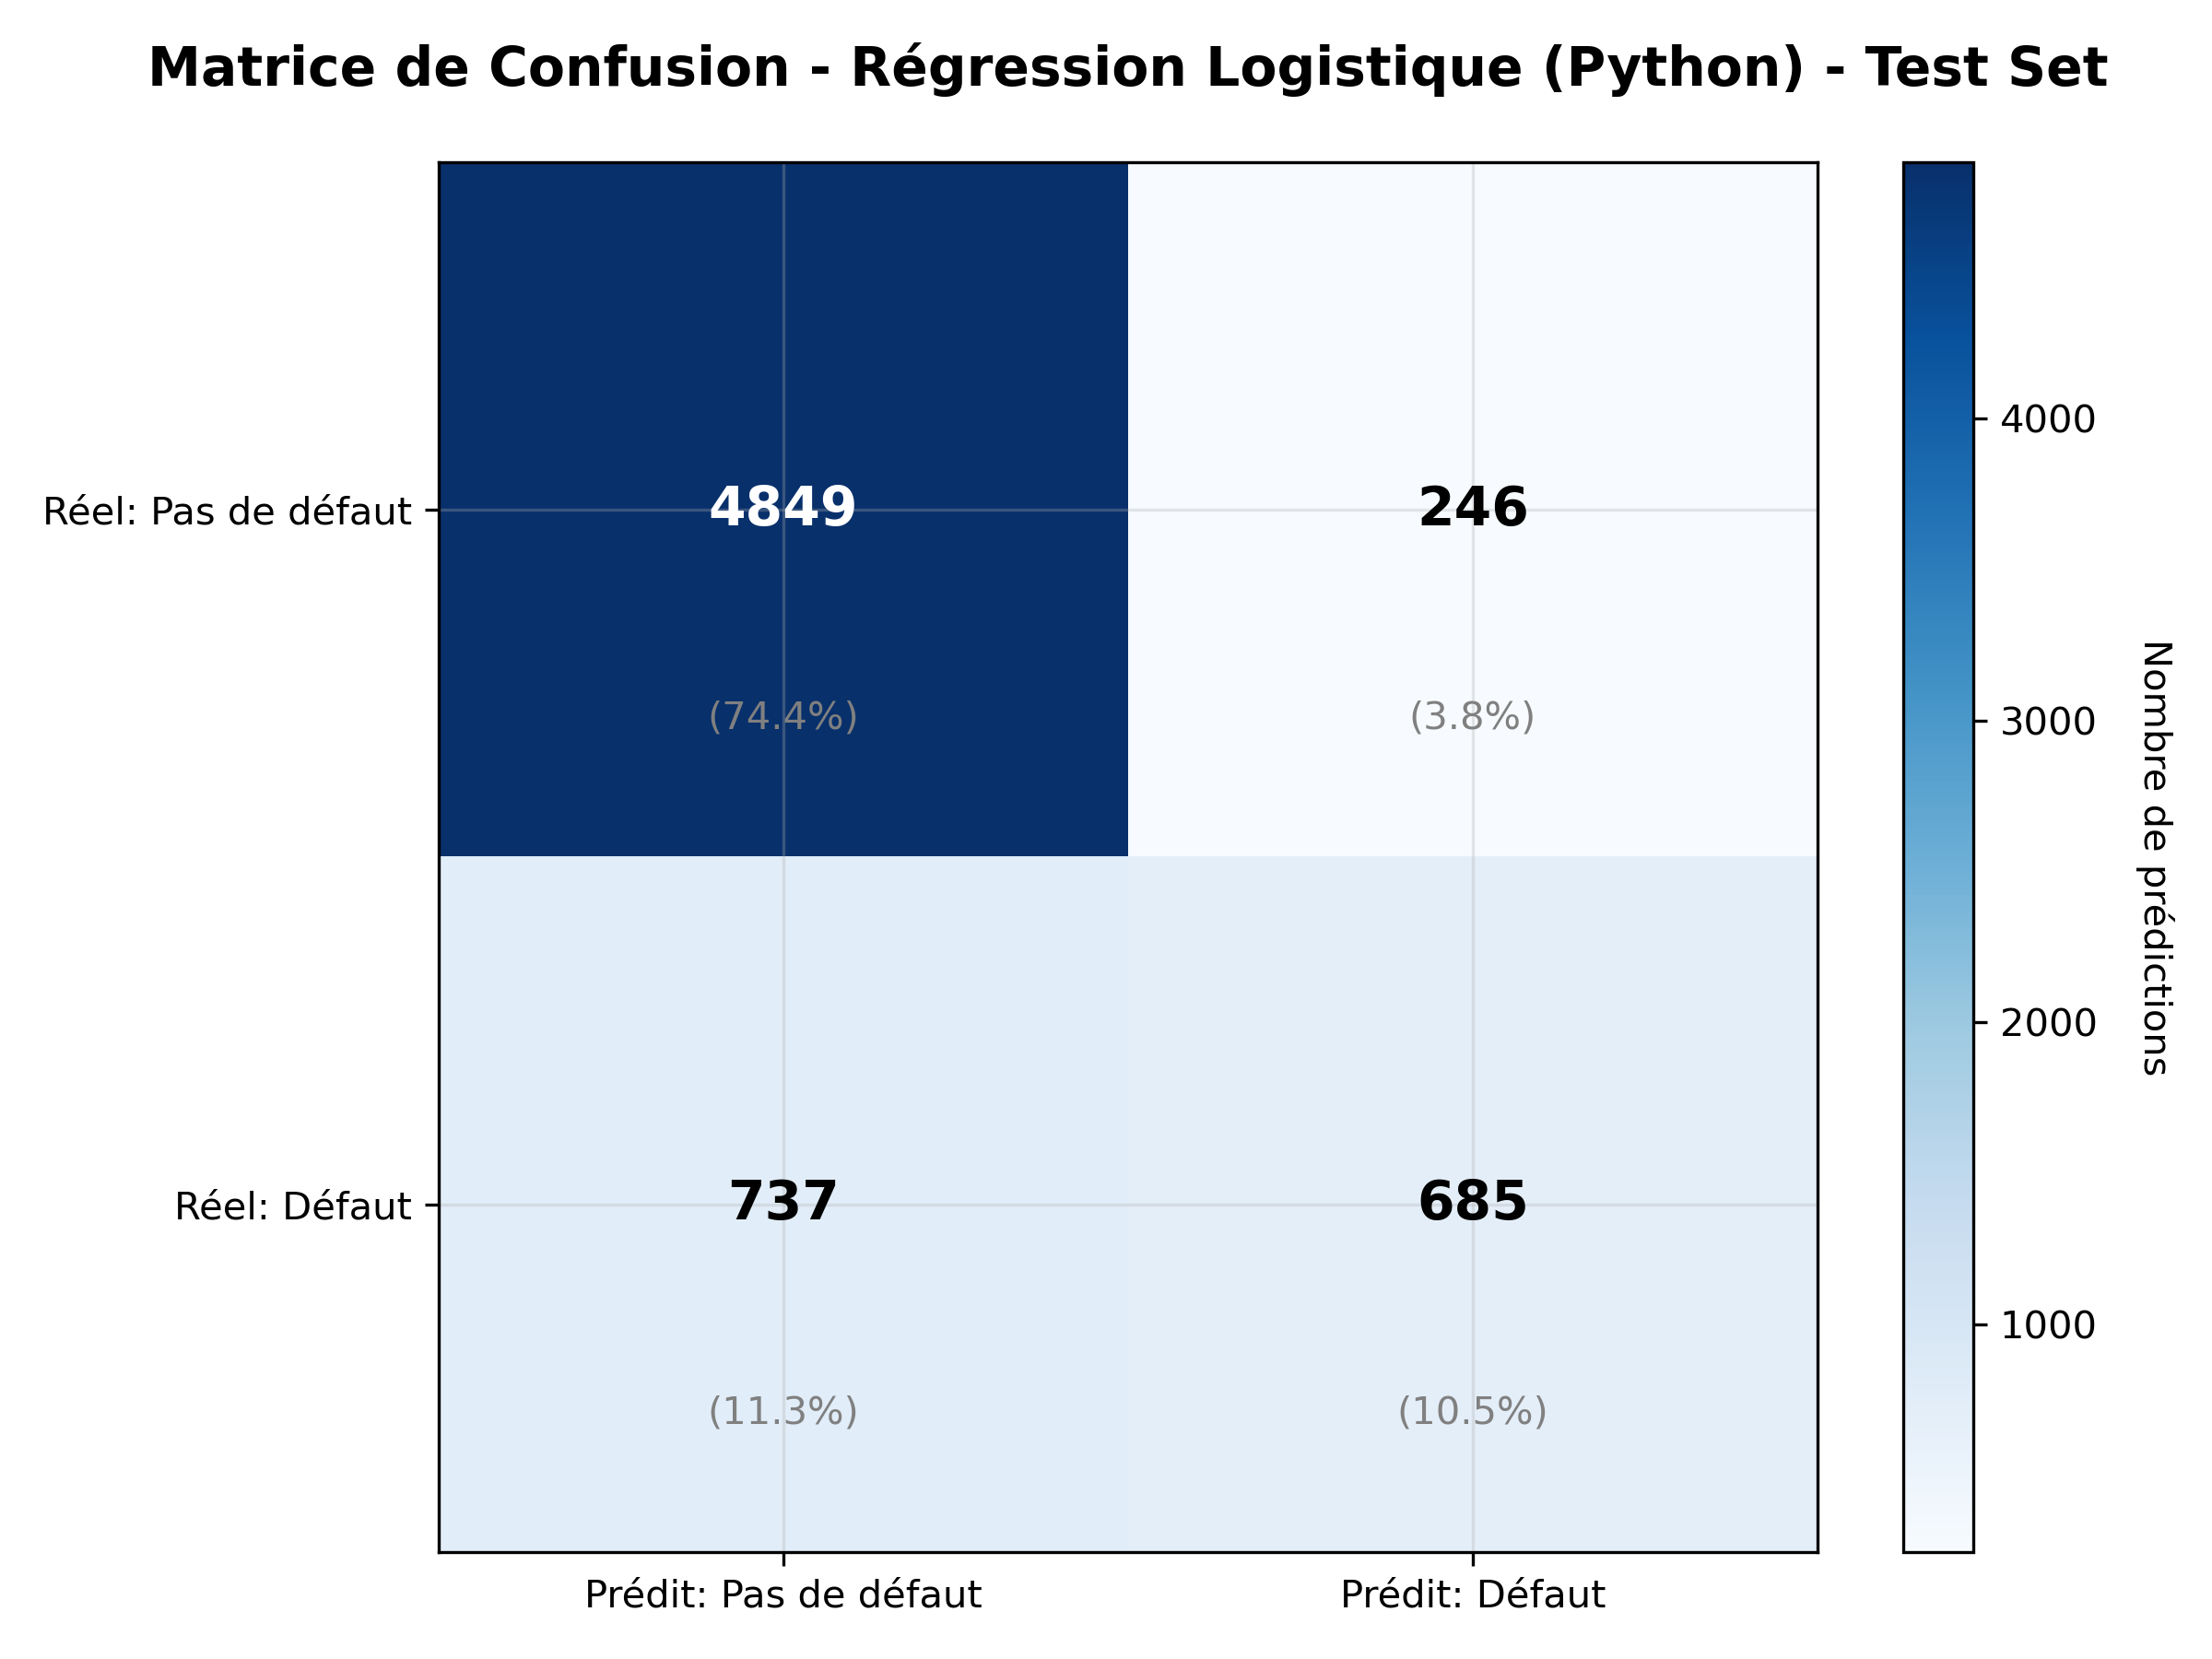
\includegraphics[width=\textwidth]{logistic_regression/lr_python_confusion_matrix_test.png}
        \caption{Matrice de confusion LR}
    \end{subfigure}
    \hfill
    \begin{subfigure}[b]{0.48\textwidth}
        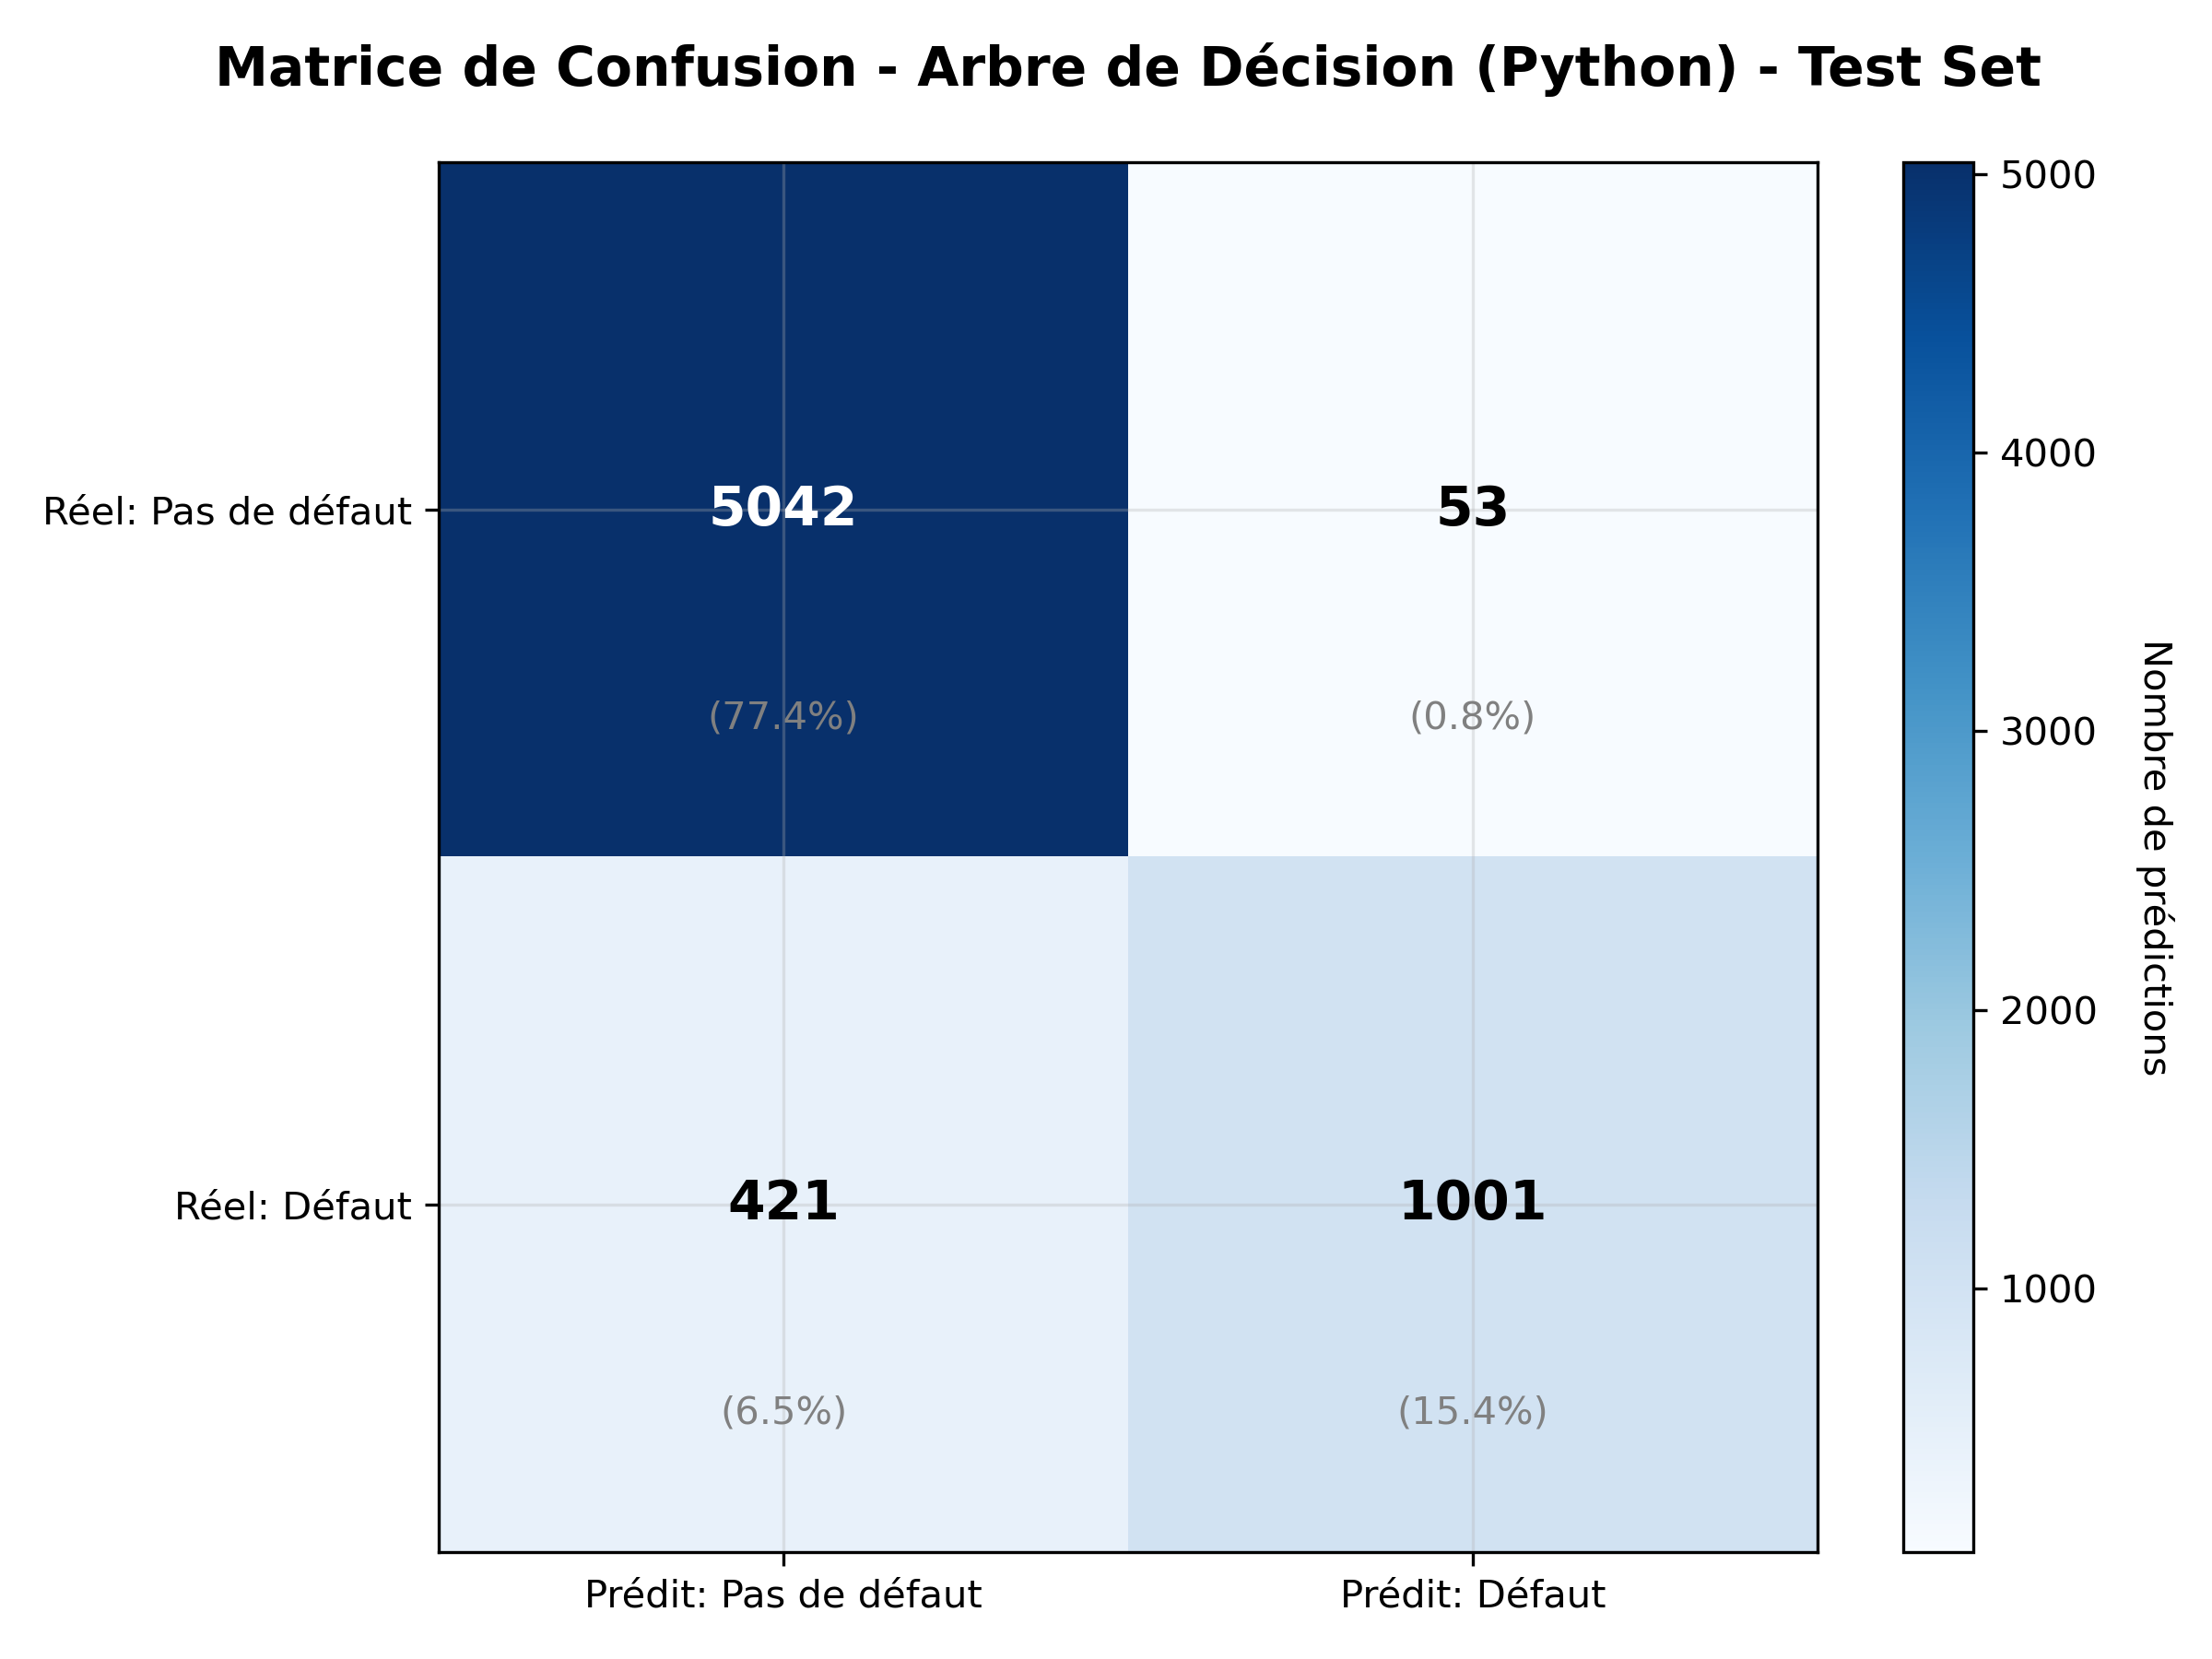
\includegraphics[width=\textwidth]{decision_tree/dt_python_confusion_matrix_test.png}
        \caption{Matrice de confusion DT}
    \end{subfigure}
    \caption{Matrices de confusion sur le test set.}
    \label{fig:confusion}
\end{figure}

\begin{figure}[H]
    \centering
    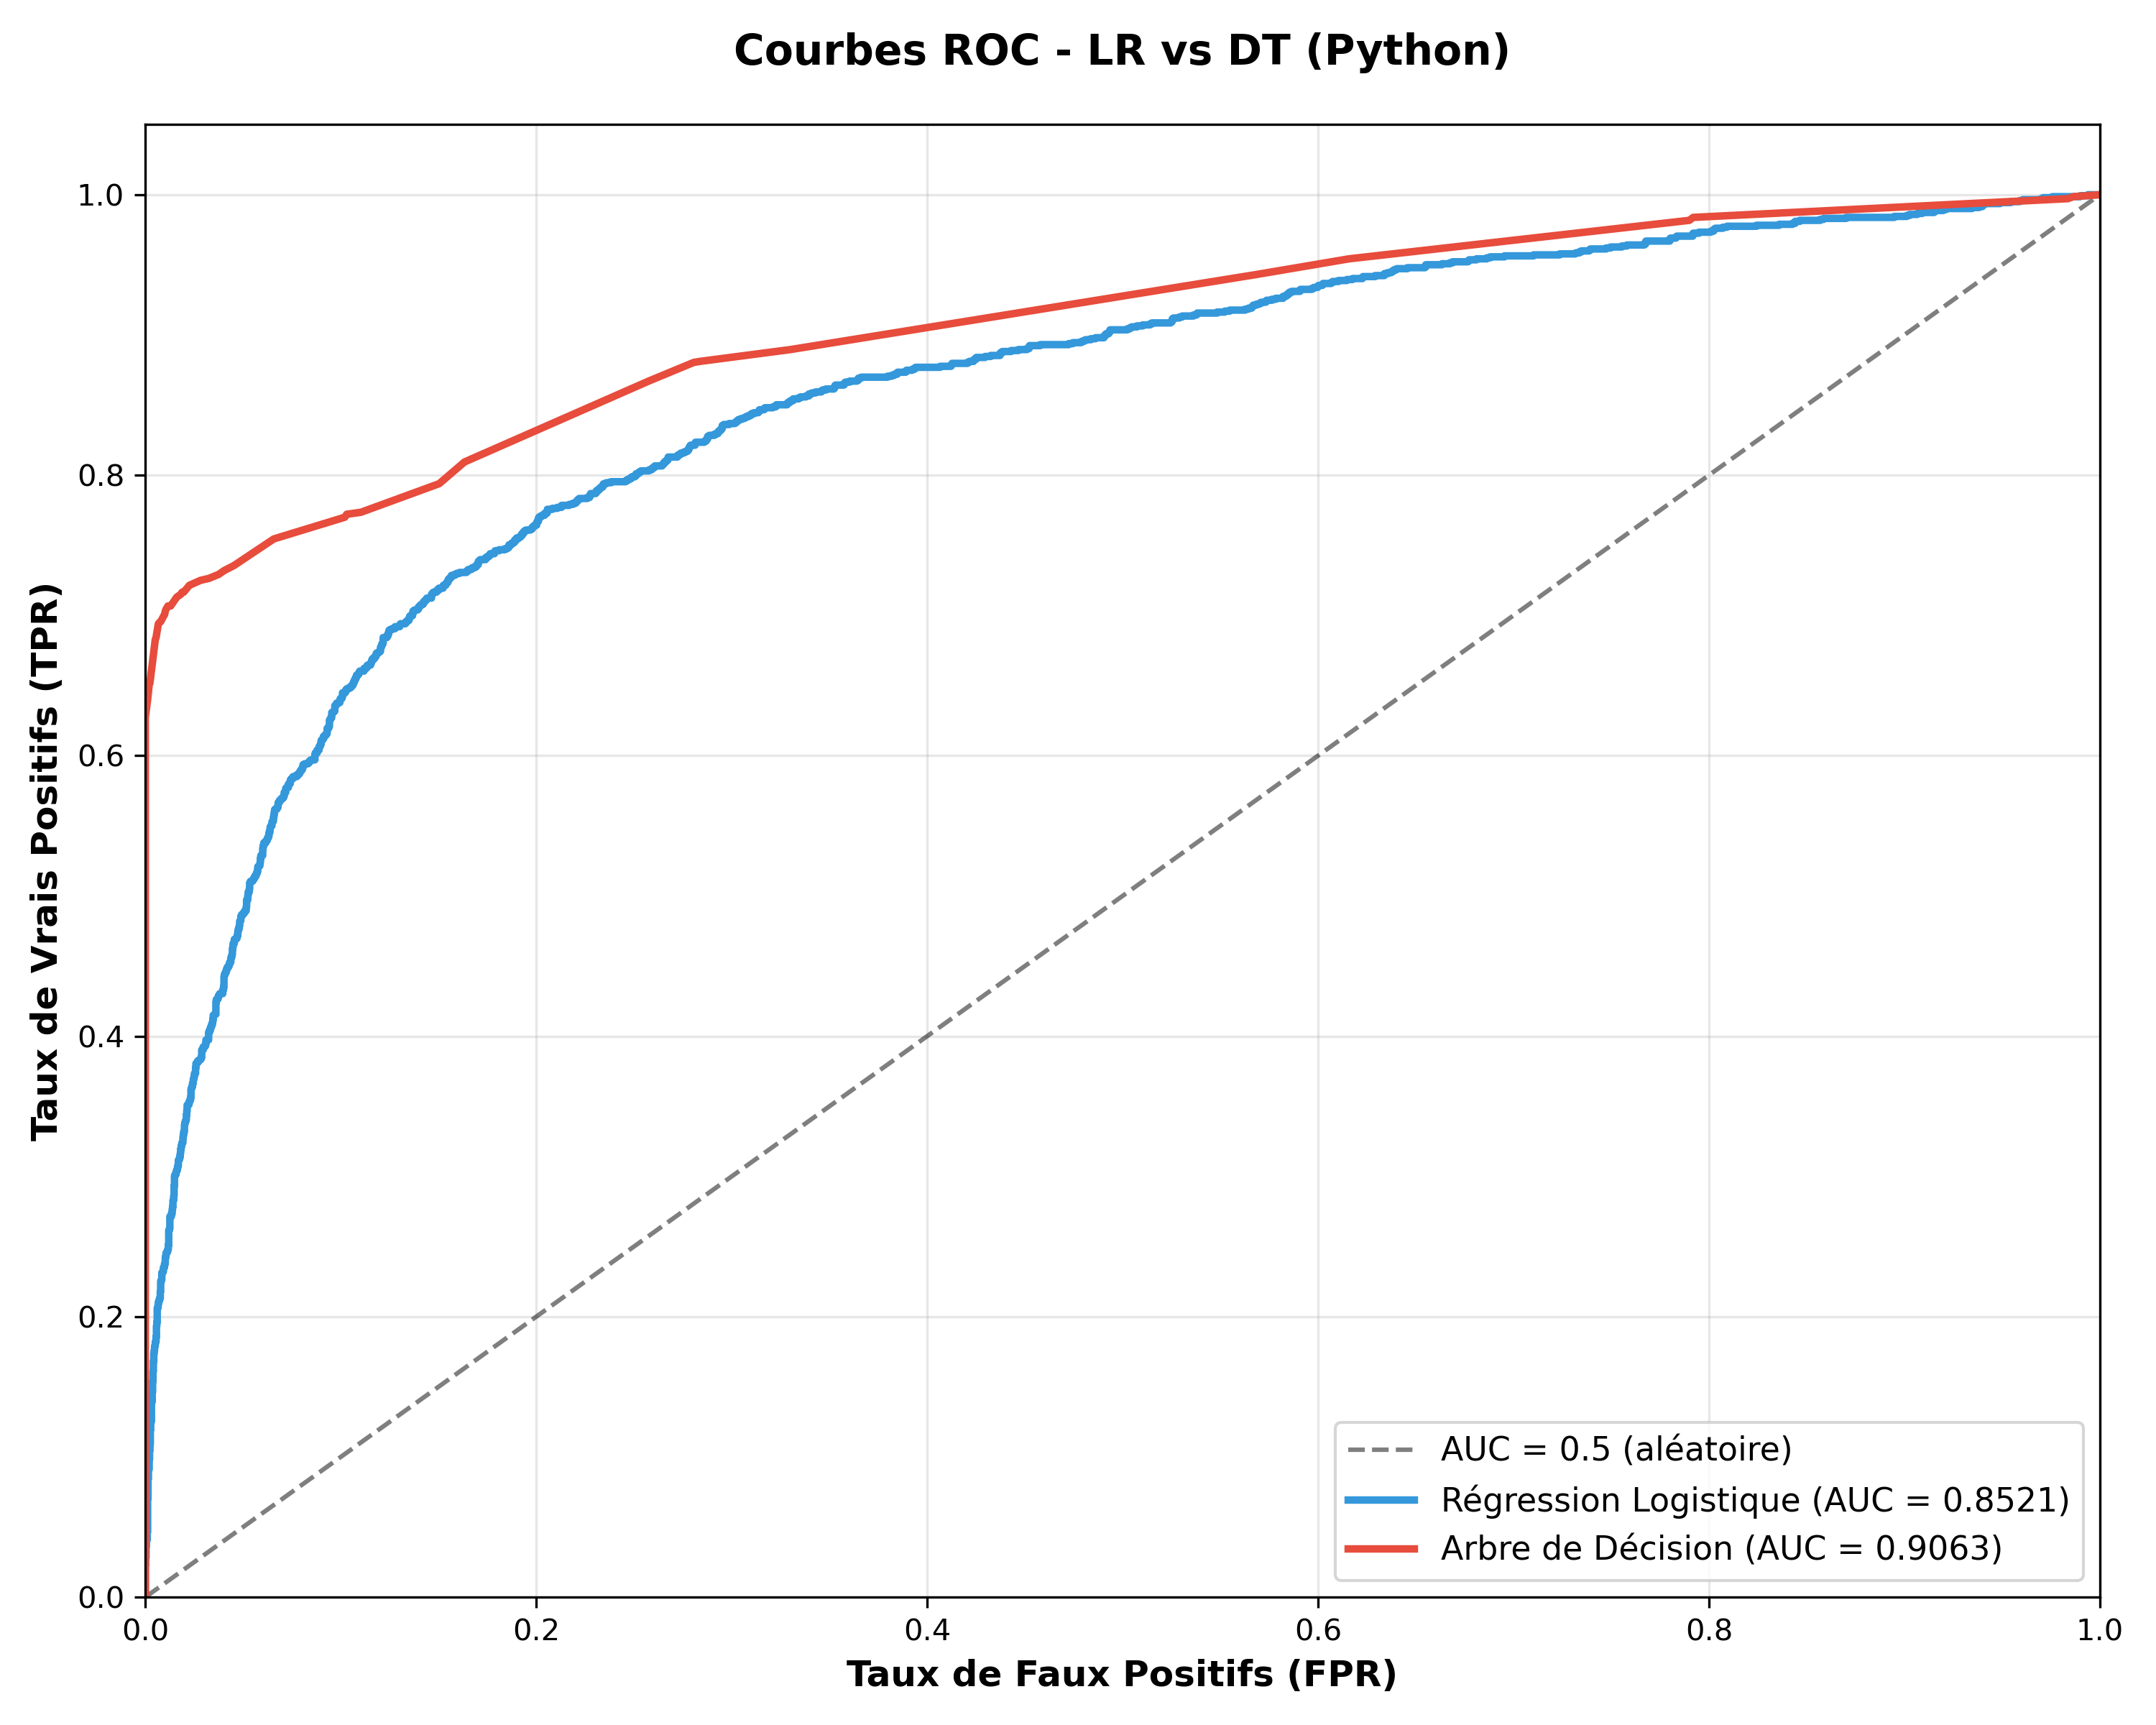
\includegraphics[width=0.78\textwidth]{logistic_regression/lr_dt_python_roc_curves_comparison.png}
    \caption{Courbes ROC : comparaison LR vs DT.}
    \label{fig:roc}
\end{figure}

\section{Seuils de décision métier}

La probabilité brute produite par chaque modèle est transformée en décision de crédit par la fonction \texttt{\_classify()} du module \file{predict.py}, selon les trois seuils définis dans le Tableau~\ref{tab:seuils}. Une probabilité de défaut inférieure à 30\,\% est considérée comme sûre et entraîne l'acceptation totale du prêt. Entre 30\,\% et 60\,\%, le profil est jugé moyennement risqué et le prêt est accepté partiellement (avec des conditions renforcées, par exemple). Au-delà de 60\,\%, le prêt est refusé. Ces seuils constituent une politique conservatrice adaptable : dans un contexte réel, ils seraient calibrés en fonction de l'appétence au risque de l'établissement prêteur et du coût relatif des faux positifs et faux négatifs.

\begin{table}[H]
    \centering
    \caption{Seuils de classification métier}
    \label{tab:seuils}
    \begin{tabular}{l l l}
        \toprule
        \textbf{Probabilité} & \textbf{Niveau de risque} & \textbf{Décision} \\
        \midrule
        $< 0{,}30$          & Safe                      & Accepté totalement \\
        0,30 - 0,60   & Moyennement à risque      & Accepté partiellement \\
        $> 0{,}60$           & À risque                  & Refusé \\
        \bottomrule
    \end{tabular}
\end{table}


% ════════════════════════════════════════════════════════════════════════════
% CHAPITRE 4 - OUTILS ET JUSTIFICATIONS (SECTION MAJEURE)
% ════════════════════════════════════════════════════════════════════════════
\chapter{Outils et justifications}

% Grille d'analyse appliquée systématiquement :
% - Besoin couvert
% - Alternatives envisagées (2-3)
% - Critères de choix
% - Version utilisée
% - Installation / commande
% - Configuration retenue
% - Limites / risques
% - Licence

\section{Grille d'analyse}

Chaque outil est évalué selon une grille standardisée : besoin couvert, alternatives
envisagées, critères de choix, version, installation, configuration, limites et licence.
Cette approche permet une comparaison objective et justifie chaque décision technique.

\section{Langages}

\subsection{Python 3.11}
Python est utilisé pour l'ensemble du back-end : scripts d'analyse, pipeline ML et API REST. Les alternatives considérées étaient R (écosystème statistique riche mais moins adapté au développement web), Julia (performant mais écosystème moins mature) et Java (verbeux pour du prototypage ML). Python a été retenu pour son écosystème ML dominant (scikit-learn, pandas, NumPy), sa syntaxe concise et la disponibilité de frameworks web légers comme Flask. La version~3.11 est imposée par l'image Docker \texttt{python:3.11-slim}. La principale limite de Python reste le GIL (\emph{Global Interpreter Lock}), qui empêche le parallélisme CPU natif, mais ce n'est pas contraignant ici puisque les prédictions sont séquentielles et rapides. Licence : PSF License (libre).

\subsection{JavaScript (ES2022)}

JavaScript est le langage du front-end, exécuté dans le navigateur via Vue~3 et Vite. Les alternatives envisagées étaient TypeScript (typage statique, mais surcoût de configuration pour un projet de cette taille), Dart via Flutter~Web (écosystème encore restreint côté web) et Streamlit (Python, mais limité en personnalisation d'interface). JavaScript ES2022 a été retenu pour sa compatibilité native avec l'écosystème Vue/Vite et l'absence de phase de compilation. La version est déterminée par Node~20 (image Docker \texttt{node:20-alpine}). La principale limite est l'absence de typage statique, qui pourrait compliquer la maintenance sur un projet plus large.

\section{Pipeline ML}

\subsection{scikit-learn}
Scikit-learn~\cite{scikit-learn} fournit l'ensemble des fonctionnalités ML du projet : entraînement des modèles (\texttt{LogisticRegression}, \texttt{DecisionTreeClassifier}), normalisation (\texttt{StandardScaler}), split stratifié (\texttt{train\_test\_split}) et métriques d'évaluation (\texttt{accuracy\_score}, \texttt{f1\_score}, \texttt{roc\_auc\_score}, etc.). Les alternatives considérées étaient TensorFlow et PyTorch (surdimensionnés pour des modèles classiques sans deep learning), XGBoost et LightGBM (pertinents mais introduisant une dépendance supplémentaire pour un gain incertain sur ce dataset). Scikit-learn a été retenu pour la cohérence de son API, sa documentation exhaustive et son adéquation avec des modèles interprétables. Version~$\geq$~1.2.0, licence BSD-3-Clause. Limite : pas de support GPU ni de modèles profonds.

\subsection{pandas / NumPy}

Pandas~\cite{pandas} et NumPy~\cite{numpy} assurent respectivement la manipulation des données tabulaires (chargement CSV, filtrage, agrégation) et les opérations numériques sur les tableaux multidimensionnels. Les alternatives étaient Polars (plus rapide sur les gros volumes, mais interopérabilité moindre avec scikit-learn) et Dask (calcul distribué, non nécessaire ici avec 32\,581 lignes). Ces deux bibliothèques constituent le socle standard de l'écosystème Python pour la data science. Versions~$\geq$~1.5.0 et $\geq$~1.23.0, licence BSD-3-Clause.

\subsection{matplotlib / seaborn}

Matplotlib~\cite{matplotlib} est utilisé pour générer les neuf graphiques du pipeline (matrices de confusion, courbes ROC, comparaisons de métriques, figures de synthèse). Seaborn~\cite{seaborn} complète matplotlib pour les visualisations statistiques du script d'exploration (distributions, corrélations, heatmaps). Les alternatives Plotly et Bokeh offrent de l'interactivité, mais le projet nécessite uniquement des exports PNG statiques pour le rapport et les résultats sauvegardés. Versions~$\geq$~3.6.0 et $\geq$~0.12.0.

\subsection{joblib}

Joblib~\cite{joblib} sérialise les modèles entraînés et le scaler au format \texttt{.joblib}, un format binaire optimisé pour les objets contenant de grands tableaux NumPy. Les alternatives étaient \texttt{pickle} (standard Python, mais moins performant sur les objets NumPy), ONNX (interopérable multi-langages, mais complexe à mettre en place pour des modèles scikit-learn simples) et PMML (format XML verbeux, peu utilisé en pratique). Joblib est la méthode recommandée par la documentation scikit-learn pour la persistance des modèles. Version~$\geq$~1.3.0 (dépendance transitive de scikit-learn), licence BSD-3-Clause. Limite principale : format Python-only, ce qui rend les modèles non utilisables directement depuis un autre langage.

\section{API back-end}

\subsection{Flask}
Flask~\cite{flask} est un micro-framework WSGI qui fournit le routage HTTP, la gestion des blueprints et les handlers d'erreur, sans imposer de couche d'abstraction base de données ni de validation intégrée. L'alternative principale était FastAPI, qui offre une validation automatique via Pydantic et le support natif de l'asynchrone. Flask a été préféré pour sa maturité, sa simplicité de configuration (un seul blueprint suffit pour les quatre routes du projet) et le fait que les prédictions scikit-learn sont des opérations synchrones rapides ne nécessitant pas d'async. Django REST Framework a été écarté car trop lourd pour une API de quatre endpoints. Version~$\geq$~3.0.0, licence BSD-3-Clause. Configuration retenue : CORS ouvert (\texttt{origins="*"}), Gunicorn en production.

\subsection{Marshmallow}

Marshmallow~\cite{marshmallow} assure la validation et la désérialisation des payloads JSON entrants. Le schéma \texttt{PredictionInputSchema} déclare les types, les bornes (âge entre 18 et 100, taux d'intérêt entre 0 et 30) et les valeurs catégorielles autorisées. L'alternative Pydantic est plus moderne et offre une validation similaire, mais Marshmallow a été choisi pour sa compatibilité historique avec Flask et la distinction claire entre schémas de validation (entrée) et de sérialisation (sortie). Version~$\geq$~3.0.0, licence MIT.

\subsection{SQLAlchemy}

SQLAlchemy~\cite{sqlalchemy} est utilisé comme ORM pour persister les prédictions. Le modèle \texttt{Prediction} déclare une table contenant les 11~features d'entrée, le modèle utilisé et les résultats (probabilité, niveau de risque, décision) pour LR et DT. L'intérêt principal de SQLAlchemy est son support multi-moteurs : en développement et en tests, l'application utilise SQLite (y compris en mémoire pour les tests), tandis qu'en production Docker, elle se connecte à PostgreSQL via la variable \texttt{DATABASE\_URL}. Ce changement de backend ne nécessite aucune modification de code. Alternatives écartées : Peewee (moins de fonctionnalités), Django ORM (lié au framework Django). Version~$\geq$~2.0.0, licence MIT.

\subsection{Gunicorn}

Gunicorn~\cite{gunicorn} est le serveur WSGI utilisé en production pour servir l'application Flask. Il remplace le serveur de développement intégré à Flask, qui n'est pas conçu pour gérer la concurrence. Le Dockerfile de l'API le lance avec \texttt{gunicorn -{}-bind 0.0.0.0:8000 app.main:app}. Les alternatives étaient uWSGI (plus configurable mais plus complexe) et Waitress (portable sur Windows, non pertinent ici). Version~$\geq$~21.0.0, licence MIT.

\subsection{Flask-CORS / psycopg2-binary}

Flask-CORS~\cite{flaskcors} active le partage de ressources entre origines (CORS) pour permettre au front-end, servi sur le port~5173, d'appeler l'API sur le port~8000. La configuration actuelle autorise toutes les origines (\texttt{origins="*"}), ce qui est acceptable en développement mais devrait être restreint en production. Psycopg2-binary~\cite{psycopg2} est le driver PostgreSQL utilisé par SQLAlchemy pour communiquer avec la base de données en production Docker. La variante \texttt{-binary} inclut les bibliothèques C pré-compilées, évitant la nécessité de compiler \texttt{libpq} dans le conteneur.

\section{Front-end}

\subsection{Vue 3}
Vue~3~\cite{vuejs} est le framework JavaScript retenu pour l'interface utilisateur. Il fournit un système de composants réactifs, une Composition~API concise et des Single~File~Components (\texttt{.vue}) qui regroupent template, script et style dans un même fichier. Les alternatives considérées étaient React (écosystème plus vaste mais JSX moins lisible pour un projet de cette taille), Svelte (compilateur innovant mais communauté plus restreinte) et Angular (framework complet mais lourd pour quatre vues). Vue~3 a été retenu pour sa courbe d'apprentissage modérée et sa légèreté. L'application n'utilise pas de state manager (Pinia) car l'état est local à chaque vue. Version~$\geq$~3.5.25, licence MIT.

\subsection{Vite}

Vite~\cite{vite} est le bundler et serveur de développement du front-end. Il remplace Webpack en proposant un démarrage quasi instantané grâce au \emph{native ESM} et un rechargement à chaud (HMR) très rapide. La configuration est minimale : le fichier \file{vite.config.js} déclare les plugins Vue et Tailwind, et ouvre le serveur sur \texttt{0.0.0.0} pour être accessible depuis l'hôte Docker. Les alternatives Webpack (configuration complexe) et Parcel (moins de contrôle sur les plugins) ont été écartées. Version~$\geq$~7.3.1, licence MIT.

\subsection{Tailwind CSS 4}

Tailwind~CSS~\cite{tailwindcss} est un framework CSS \emph{utility-first} qui permet de styler les composants directement dans le HTML via des classes utilitaires (\texttt{bg-white}, \texttt{rounded-lg}, \texttt{px-4}). Cette approche élimine le besoin d'écrire des fichiers CSS dédiés et garantit la cohérence visuelle. Les alternatives Bootstrap (composants prédéfinis, moins flexible) et CSS vanilla (effort de maintenance supérieur) ont été écartées. L'intégration avec Vite se fait via le plugin \texttt{@tailwindcss/vite} déclaré dans la configuration. Version~$\geq$~4.1.18, licence MIT.

\subsection{Vue Router 4}

Vue~Router~\cite{vuerouter} gère la navigation côté client entre les trois routes de l'application : \texttt{/} (formulaire de prédiction), \texttt{/history} (liste des prédictions) et \texttt{/history/:id} (détail). Le routeur utilise le mode \texttt{createWebHistory} pour des URL propres sans hash. Aucune garde d'authentification n'est configurée. Version~$\geq$~4.6.4, licence MIT.

\section{Infrastructure}

\subsection{Docker / Docker Compose}
Docker~\cite{docker} et Docker~Compose~\cite{dockercompose} assurent la conteneurisation de l'application. Le projet utilise trois Dockerfiles distincts : un pour le pipeline ML (\texttt{python:3.11-slim} avec Make installé), un pour l'API (\texttt{python:3.11-slim} avec Gunicorn) et un pour le front-end (\texttt{node:20-alpine} avec Vite). Docker~Compose orchestre les trois services et gère le réseau inter-conteneurs. L'alternative Podman est compatible mais moins répandue en environnement académique. Vagrant a été écarté car il virtualise un OS complet, ce qui est plus lourd que la conteneurisation. Limites : le surcoût mémoire des conteneurs et la complexité du réseau Docker (résolution DNS entre services). Licence Apache~2.0.

\subsection{PostgreSQL 16}

PostgreSQL~\cite{postgresql} est la base de données relationnelle utilisée en production pour persister les prédictions. L'image Docker \texttt{postgres:16-alpine} est légère et démarre rapidement. La base \texttt{credit\_risk} est créée automatiquement au premier démarrage via les variables d'environnement du Compose. Les alternatives considérées étaient MySQL (moins de fonctionnalités SQL avancées), MongoDB (non pertinent pour des données tabulaires structurées) et SQLite en production (pas de gestion de concurrence). PostgreSQL offre la robustesse, le support des transactions ACID et une intégration native avec SQLAlchemy via psycopg2. Licence PostgreSQL (permissive, type MIT).

\subsection{Make}

GNU~Make~\cite{gnumake} orchestre le pipeline ML via un fichier \file{Makefile} déclarant dix cibles (voir Tableau~\ref{tab:makefile}). L'intérêt principal de Make est la gestion déclarative des dépendances entre cibles : la cible \texttt{train} dépend de \texttt{split}, et \texttt{plots} dépend de \texttt{train}. Ainsi, \cmd{make plots} exécute automatiquement les étapes préalables si nécessaire. Les alternatives étaient des scripts bash (pas de gestion de dépendances), Invoke (Python, moins standard), Snakemake (orienté bioinformatique) et DVC (versionnement de données, surdimensionné ici). Make a été retenu pour son ubiquité sur les systèmes Unix et sa syntaxe minimaliste. Licence GPL.

\section{Gestion de versions}

\subsection{Git}
Git~\cite{git} assure le versionnement du code du projet. C'est l'outil libre emblématique du développement logiciel : il trace chaque modification (auteur, contenu, date), permet de revenir à un état antérieur en cas de régression, et structure le travail en commits atomiques dont les messages documentent l'évolution du projet. Son modèle décentralisé permet de travailler hors ligne et fait de chaque clone une sauvegarde complète de l'historique. Les alternatives considérées étaient Subversion (SVN, centralisé : un serveur unique constitue un point de défaillance et le travail hors ligne est limité) et Mercurial (décentralisé et ergonomique, mais communauté et écosystème plus restreints). Git a été retenu pour son statut de standard de fait, son intégration native avec les forges logicielles (GitHub, GitLab) et la richesse de son outillage. Licence : GPLv2, une licence libre \emph{copyleft} - les redistributions de Git lui-même doivent rester sous GPL, ce qui ne concerne en rien le code versionné avec l'outil. Limite assumée : l'historique du projet est encore réduit, le versionnement ayant été mis en place tardivement ; des commits plus réguliers et plus fins au fil du développement auraient mieux documenté la démarche, et c'est la pratique adoptée pour les corrections récentes du projet.

\section{Tests et qualité}

\subsection{pytest}
Pytest~\cite{pytest} est le framework de tests du projet, configuré via \file{pytest.ini} avec les options \texttt{-v -{}-tb=short} pour un affichage détaillé et des tracebacks concis. Pytest a été préféré au module standard \texttt{unittest} pour sa syntaxe plus concise (simples fonctions \texttt{assert} au lieu de méthodes de classe), son système de fixtures (utilisé pour le client Flask de test) et sa découverte automatique des fichiers \texttt{test\_*.py}. L'alternative \texttt{nose2} est en déclin. Version~$\geq$~7.0.0, licence MIT.

\subsection{SQLite in-memory}

L'isolation des tests est assurée par une base SQLite en mémoire. Le fichier \file{conftest.py} définit \texttt{DATABASE\_URL=sqlite:///:memory:} avant tout import de l'application, ce qui force SQLAlchemy à utiliser une base éphémère créée à chaque session de tests. Cette approche élimine la dépendance à PostgreSQL pour l'exécution des tests et garantit que chaque lancement part d'un état vierge. Le flag \texttt{check\_same\_thread=False} est activé dans la configuration de l'engine pour permettre l'utilisation de SQLite dans un contexte multi-thread Flask.

\subsection{pytest-cov}

Pytest-cov~\cite{pytest-cov} mesure la couverture de code des tests, c'est-à-dire la proportion de lignes du module \file{app/} effectivement exécutées par la suite de tests. La cible \cmd{make coverage} produit un rapport ligne à ligne dans le terminal (option \texttt{-{}-cov-report=term-missing}), qui identifie les branches non testées. La mesure actuelle s'établit à 97\,\% sur le module de l'API ; elle ne couvre ni les scripts ML ni le front-end (voir chapitre~6). L'alternative consistant à utiliser \texttt{coverage.py} seul a été écartée au profit du plugin pytest, qui s'intègre à la suite existante sans configuration supplémentaire. Licence MIT.

\section{Tableau récapitulatif}

{\footnotesize
\newcolumntype{R}[1]{>{\raggedright\arraybackslash}p{#1}}
\begin{longtable}{R{2cm} R{2cm} R{1.2cm} R{3cm} R{2cm} R{1.2cm}}
    \caption{Tableau récapitulatif des outils} \label{tab:outils} \\
    \toprule
    \textbf{Outil} & \textbf{Rôle} & \textbf{Vers.} & \textbf{Justification} & \textbf{Altern.} & \textbf{Lic.} \\
    \midrule
    \endfirsthead
    \toprule
    \textbf{Outil} & \textbf{Rôle} & \textbf{Vers.} & \textbf{Justification} & \textbf{Altern.} & \textbf{Lic.} \\
    \midrule
    \endhead
    \midrule
    \multicolumn{6}{r}{\textit{Suite page suivante}} \\
    \endfoot
    \bottomrule
    \endlastfoot
    % Langages
    Python        & Scripts, API           & 3.11   & Écosyst. ML          & R, Julia  & PSF \\
    JavaScript    & Front-end              & ES2022 & Standard web         & TypeScript& - \\
    \midrule
    % Pipeline ML
    scikit-learn  & ML (LR, DT)            & $\geq$1.2  & API cohérente    & XGBoost   & BSD-3 \\
    pandas        & DataFrames             & $\geq$1.5  & Standard sklearn & Polars    & BSD-3 \\
    numpy         & Calculs num.           & $\geq$1.23 & Dépend. fond.    & -       & BSD-3 \\
    matplotlib    & Graphiques             & $\geq$3.6  & Export PNG       & Plotly    & PSF \\
    seaborn       & Visu. stats            & $\geq$0.12 & Heatmaps         & Plotly    & BSD-3 \\
    joblib        & Sérialisation          & $\geq$1.3  & Optimisé numpy   & pickle    & BSD-3 \\
    \midrule
    % API
    Flask         & API REST               & $\geq$3.0  & Léger, pas d'async   & FastAPI   & BSD-3 \\
    Marshmallow   & Validation             & $\geq$3.0  & Schémas décl.   & Pydantic  & MIT \\
    SQLAlchemy    & ORM                    & $\geq$2.0  & Multi-DB        & Peewee    & MIT \\
    Gunicorn      & Serveur WSGI           & $\geq$21   & Standard prod        & uWSGI     & MIT \\
    Flask-CORS    & CORS                   & $\geq$4.0  & Intégr. Flask        & -       & MIT \\
    psycopg2      & Driver PG              & $\geq$2.9  & Standard PG          & asyncpg   & LGPL \\
    \midrule
    % Front-end
    Vue 3         & Framework SPA          & $\geq$3.5  & Composition API      & React     & MIT \\
    Vite          & Bundler                & $\geq$7.3  & HMR rapide    & Webpack   & MIT \\
    Tailwind      & CSS utilitaire         & $\geq$4.1  & Responsive  & Bootstrap  & MIT \\
    Vue Router    & Routing                & $\geq$4.6  & Standard Vue                   & -               & MIT \\
    \midrule
    % Infrastructure
    Docker        & Conteneurs             & -    & Reproductibilité   & Podman   & Apache \\
    PostgreSQL    & BDD                    & 16     & SQL standard       & MySQL    & PG Lic. \\
    Make          & Pipeline               & -    & Ubiquité Unix      & Invoke   & GPL \\
    Git           & Versionnement          & -    & Standard de fait   & Mercurial & GPLv2 \\
    \midrule
    % Tests
    pytest        & Tests                  & $\geq$7.0  & Fixtures, assertions   & unittest   & MIT \\
    pytest-cov    & Couverture             & $\geq$4.0  & Intégr. pytest    & coverage.py & MIT \\
\end{longtable}
}

\section{Licence du projet}

L'analyse des licences des dépendances pose naturellement la question de la licence du projet lui-même. Le code est publié sous licence MIT~\cite{mit-license} (fichier \file{LICENSE} à la racine du dépôt) : une licence libre permissive, courte et largement comprise, qui autorise la réutilisation, la modification et la redistribution du code - y compris dans un cadre propriétaire - sous seule condition de conserver la notice de copyright. Ce choix est adapté à un projet académique destiné à être lu, réutilisé et prolongé.

Il est juridiquement compatible avec l'ensemble des dépendances : les bibliothèques intégrées à l'application (Flask, scikit-learn, Vue, etc.) sont sous licences permissives (BSD, MIT, Apache~2.0, PSF), qui n'imposent aucune contrainte de licence au code qui les utilise. Les licences copyleft présentes dans le projet ne s'appliquent pas davantage au code : la GPL de Make et la GPLv2 de Git concernent les outils eux-mêmes (utilisés respectivement comme orchestrateur de build et comme gestionnaire de versions, sans lien de code avec l'application), et la LGPL de psycopg2 autorise expressément l'utilisation par liaison dynamique sans étendre ses obligations au programme appelant. Utiliser des outils libres n'impose donc pas leur licence au projet - c'est précisément la distinction entre licences permissives et licences copyleft que ce choix illustre.


% ════════════════════════════════════════════════════════════════════════════
% CHAPITRE 5 - ENVIRONNEMENT ET REPRODUCTIBILITÉ
% ════════════════════════════════════════════════════════════════════════════
\chapter{Environnement et reproductibilité}

\section{Installation locale}

L'installation locale nécessite Python~3.8+ (3.11 recommandé), pip et Node.js~20+. Après clonage du dépôt, un environnement virtuel Python est créé pour isoler les dépendances. Deux fichiers \texttt{requirements.txt} sont installés : celui du répertoire \file{back-end/} pour les scripts ML (pandas, numpy, matplotlib, seaborn, scikit-learn) et celui de \file{back-end/app/} pour l'API (Flask, SQLAlchemy, Marshmallow, Gunicorn, etc.). Le front-end est installé séparément via \texttt{npm install}. Le pipeline complet est ensuite exécuté par \cmd{make all}. Les Tableaux~\ref{tab:deps-python-scripts}, \ref{tab:deps-python-api} et~\ref{tab:deps-node} détaillent les dépendances et leurs versions minimales.

\begin{lstlisting}[style=bash, caption={Installation et exécution du pipeline}]
# Cloner et preparer l'environnement
git clone <url-du-repo>
cd PROGRAMME
python3 -m venv .venv
source .venv/bin/activate
pip install -r back-end/requirements.txt
pip install -r back-end/app/requirements.txt

# Pipeline ML complet
make all        # split -> train -> plots

# Tests
make test       # 25 tests pytest

# Front-end (developpement local)
cd front-end
npm install
npm run dev     # http://localhost:5173
\end{lstlisting}

\section{Déploiement Docker}

Le déploiement Docker requiert au préalable l'exécution de \cmd{make train} pour générer les modèles \texttt{.joblib}, qui sont copiés dans l'image de l'API au moment du build ; la cible \cmd{make docker-up} enchaîne automatiquement ces deux étapes dans le bon ordre. Si les modèles manquent malgré tout, l'API refuse de démarrer avec un message explicite indiquant la commande à lancer, plutôt qu'une erreur confuse. La commande \texttt{docker compose up -d -{}-build} construit les trois images et démarre les conteneurs dans l'ordre garanti par les healthchecks (PostgreSQL prêt avant l'API, API saine avant le front-end). Le service PostgreSQL est exposé sur le port~5433 de la machine hôte (5432 à l'intérieur du réseau Docker), afin d'éviter tout conflit avec un éventuel PostgreSQL déjà installé localement ; l'API est accessible sur le port~8000 et l'interface web sur le port~5173. La vérification se fait via \texttt{curl http://localhost:8000/health}, qui retourne \texttt{\{"status": "ok"\}} si l'API est opérationnelle.

\begin{lstlisting}[style=bash, caption={Déploiement avec Docker Compose}]
# Prerequis : make train (modeles .joblib requis)
make train

# Lancer les 3 services
docker compose up -d --build

# Verifier
curl http://localhost:8000/health    # {"status": "ok"}
# Interface web : http://localhost:5173

# Arreter
docker compose down
\end{lstlisting}

\section{Exécution du pipeline}

Le Tableau~\ref{tab:makefile} récapitule les douze cibles du Makefile. La chaîne principale \texttt{all} enchaîne \texttt{split}, \texttt{train} et \texttt{plots}. Les cibles \texttt{explore} et \texttt{outliers} sont indépendantes et peuvent être exécutées à tout moment pour analyser les données brutes. La cible \texttt{test} dépend de \texttt{train} car les tests d'intégration de l'API nécessitent les modèles sérialisés pour effectuer des prédictions. Enfin, \texttt{clean} supprime l'ensemble des fichiers générés (résultats, modèles, données traitées), permettant de repartir d'un état vierge.

\begin{table}[H]
    \centering
    \caption{Cibles du Makefile}
    \label{tab:makefile}
    \begin{tabularx}{\textwidth}{l l X}
        \toprule
        \textbf{Commande} & \textbf{Dépendance} & \textbf{Description} \\
        \midrule
        \cmd{make all}         & split, train, plots  & Pipeline complet \\
        \cmd{make split}       & -                  & Split stratifié 80/20 du dataset \\
        \cmd{make train}       & split                & Entraînement LR + DT, sauvegarde .joblib \\
        \cmd{make train-force} & split                & Réentraînement forcé (ignore le cache) \\
        \cmd{make plots}       & train                & Génération des 9 graphiques \\
        \cmd{make explore}     & -                  & Exploration statistique des données \\
        \cmd{make outliers}    & -                  & Détection des outliers (IQR + Z-score) \\
        \cmd{make test}        & train                & 25 tests pytest \\
        \cmd{make coverage}    & train                & Tests avec couverture (pytest-cov) \\
        \cmd{make docker-up}   & train                & Entraînement puis docker compose up \\
        \cmd{make clean}       & -                  & Suppression des fichiers générés \\
        \cmd{make help}        & -                  & Affiche l'aide \\
        \bottomrule
    \end{tabularx}
\end{table}

\section{Tableau des versions}

Les tableaux suivants listent les dépendances avec leurs versions minimales requises, telles que déclarées dans les fichiers \file{requirements.txt} et \file{package.json}. Les versions exactes installées lors du développement sont documentées dans le fichier \file{docs/Rapport final/versions\_exactes.md} (obtenues via \texttt{pip freeze} et \texttt{npm list}).

\begin{table}[H]
    \centering
    \caption{Dépendances Python (scripts ML)}
    \label{tab:deps-python-scripts}
    \begin{tabular}{l l l}
        \toprule
        \textbf{Package} & \textbf{Version min.} & \textbf{Rôle} \\
        \midrule
        pandas        & $\geq$ 1.5.0  & Manipulation de données \\
        numpy         & $\geq$ 1.23.0 & Calculs numériques \\
        matplotlib    & $\geq$ 3.6.0  & Graphiques \\
        seaborn       & $\geq$ 0.12.0 & Visualisation statistique \\
        scikit-learn  & $\geq$ 1.2.0  & ML (entraînement, métriques) \\
        \bottomrule
    \end{tabular}
\end{table}

\begin{table}[H]
    \centering
    \caption{Dépendances Python (API Flask)}
    \label{tab:deps-python-api}
    \begin{tabular}{l l l}
        \toprule
        \textbf{Package} & \textbf{Version min.} & \textbf{Rôle} \\
        \midrule
        flask            & $\geq$ 3.0.0  & Micro-framework HTTP \\
        flask-cors       & $\geq$ 4.0.0  & Gestion CORS \\
        gunicorn         & $\geq$ 21.0.0 & Serveur WSGI production \\
        marshmallow      & $\geq$ 3.0.0  & Validation de schémas \\
        sqlalchemy       & $\geq$ 2.0.0  & ORM (PostgreSQL / SQLite) \\
        psycopg2-binary  & $\geq$ 2.9.0  & Driver PostgreSQL \\
        scikit-learn     & $\geq$ 1.2.0  & Chargement des modèles \\
        joblib           & $\geq$ 1.3.0  & Désérialisation .joblib \\
        numpy            & $\geq$ 1.23.0 & Tableaux numériques \\
        pandas           & $\geq$ 1.5.0  & DataFrames (predict) \\
        pytest           & $\geq$ 7.0.0  & Tests \\
        pytest-cov       & $\geq$ 4.0.0  & Couverture de code \\
        \bottomrule
    \end{tabular}
\end{table}

\begin{table}[H]
    \centering
    \caption{Dépendances Node.js (front-end)}
    \label{tab:deps-node}
    \begin{tabular}{l l l}
        \toprule
        \textbf{Package} & \textbf{Version} & \textbf{Rôle} \\
        \midrule
        vue                  & $\geq$ 3.5.25  & Framework SPA \\
        vue-router           & $\geq$ 4.6.4   & Routing client \\
        tailwindcss          & $\geq$ 4.1.18  & CSS utilitaire \\
        @tailwindcss/vite    & $\geq$ 4.1.18  & Plugin Vite pour Tailwind \\
        \midrule
        vite (dev)           & $\geq$ 7.3.1   & Bundler / dev server \\
        @vitejs/plugin-vue (dev) & $\geq$ 6.0.2& Plugin Vue pour Vite \\
        \bottomrule
    \end{tabular}
\end{table}


% ════════════════════════════════════════════════════════════════════════════
% CHAPITRE 6 - TESTS
% ════════════════════════════════════════════════════════════════════════════
\chapter{Tests}

\section{Stratégie de tests}

La suite de tests comprend 25~cas répartis dans cinq fichiers, comme le détaille le Tableau~\ref{tab:tests}. La stratégie couvre trois niveaux : les tests unitaires vérifient les fonctions isolées (encodage des features dans \file{test\_preprocess.py}, seuils de classification dans \file{test\_predict.py}, validation des schémas Marshmallow dans \file{test\_schemas.py}, absence de fuite de données dans l'imputation du pipeline dans \file{test\_imputation.py}), tandis que les tests d'intégration dans \file{test\_api.py} exercent les endpoints REST de bout en bout, de la requête HTTP à la réponse JSON en passant par la prédiction et la persistance en base. Ce découpage permet d'identifier rapidement l'origine d'une régression : un échec dans \file{test\_preprocess.py} pointe vers un problème d'encodage, tandis qu'un échec dans \file{test\_api.py} peut impliquer n'importe quelle couche de la pile.

\begin{table}[H]
    \centering
    \caption{Répartition des tests}
    \label{tab:tests}
    \begin{tabularx}{\textwidth}{l r X}
        \toprule
        \textbf{Fichier} & \textbf{Tests} & \textbf{Couverture} \\
        \midrule
        \file{test\_api.py}        & 7 & Endpoints REST (health, predict, predictions, erreurs, bornes) \\
        \file{test\_imputation.py} & 3 & Anti-fuite : statistiques d'imputation issues du train uniquement \\
        \file{test\_predict.py}    & 5 & Seuils de classification \_classify (Safe, Moyen, Risque, limites) \\
        \file{test\_preprocess.py} & 3 & Encodage features (shape, mappings catégoriels, ordre) \\
        \file{test\_schemas.py}    & 7 & Validation Marshmallow (payload, bornes dont loan\_amnt, catégoriel, requis) \\
        \midrule
        \textbf{Total}             & \textbf{25} & \\
        \bottomrule
    \end{tabularx}
\end{table}

\section{Isolation}

L'isolation des tests repose sur deux mécanismes. D'une part, le fichier \file{conftest.py} redéfinit la variable d'environnement \texttt{DATABASE\_URL} vers \texttt{sqlite:///:memory:} \emph{avant} l'import de l'application Flask, ce qui force SQLAlchemy à créer une base éphémère en mémoire. D'autre part, la fixture \texttt{client} active le mode \texttt{TESTING} de Flask et fournit un client HTTP de test qui simule les requêtes sans ouvrir de socket réseau. Cette approche garantit que les tests s'exécutent sans dépendance externe (pas de PostgreSQL, pas de serveur HTTP) et que chaque session de tests démarre avec une base vide.

\section{Exécution}

L'exécution des tests se fait via \cmd{make test}, qui dépend de la cible \texttt{train} pour s'assurer que les modèles \texttt{.joblib} existent. Le Makefile sélectionne l'interpréteur du virtualenv (\texttt{.venv/bin/python}) s'il existe, et \texttt{python3} du système sinon. Lors de la dernière exécution, les 25~tests passent avec succès en moins d'une seconde, confirmant l'absence de régression sur la validation des entrées, l'encodage des features, l'imputation, les seuils de classification et les quatre endpoints de l'API.

\section{Couverture de code}

La couverture de code, mesurée par pytest-cov via \cmd{make coverage}, s'établit à 97\,\% des 193~instructions du module \file{app/} (les cinq lignes non couvertes correspondent au handler d'erreur 500 et au message d'absence des modèles). Cette mesure doit être interprétée avec prudence : elle porte uniquement sur le code de l'API - les scripts du pipeline ML ne sont couverts qu'indirectement par \file{test\_imputation.py} et le front-end Vue ne dispose d'aucun test automatisé - et une ligne exécutée n'est pas pour autant une ligne correctement vérifiée. Elle fournit néanmoins un indicateur objectif pour repérer les zones non testées.


% ════════════════════════════════════════════════════════════════════════════
% CHAPITRE 7 - LIMITES ET AMÉLIORATIONS
% ════════════════════════════════════════════════════════════════════════════
\chapter{Limites et améliorations}

\section{Limites actuelles}

Plusieurs limites identifiées découlent des choix de simplification évoqués en introduction. Sur le plan de la sécurité, l'API est publique (pas d'authentification), la politique CORS autorise toutes les origines (\texttt{origins="*"}), et les identifiants de la base PostgreSQL sont écrits en clair dans \file{docker-compose.yml}. Sur le plan méthodologique, la profondeur de l'arbre est désormais choisie par validation croisée à 5~plis, mais l'évaluation finale repose toujours sur un unique split 80/20 : des intervalles de confiance (validation croisée imbriquée ou bootstrap) rendraient les métriques moins sensibles à la partition aléatoire. Le déséquilibre des classes (78/22\,\%) a été quantifié à travers les variantes \texttt{class\_weight="balanced"} (Tableau~\ref{tab:class-weight}) ; le modèle déployé reste néanmoins la version non pondérée, et les techniques de rééchantillonnage comme SMOTE n'ont pas été explorées. Sur le plan opérationnel, le projet dispose d'une mesure de couverture mais pas d'intégration continue : les tests sont exécutés manuellement via \cmd{make test}. Il n'y a pas non plus de monitoring ni de logging structuré, et le conteneur front-end utilise le serveur de développement Vite au lieu d'un build de production servi par un serveur statique. Enfin, le schéma de la base de données n'est pas versionné (pas d'Alembic), ce qui compliquerait l'évolution du modèle \texttt{Prediction}.

\section{Améliorations possibles}

Plusieurs axes d'amélioration concrets se dégagent. La mise en place d'une intégration continue (GitHub Actions ou GitLab CI) automatiserait l'exécution des tests, le linting et la construction des images Docker à chaque modification du dépôt. L'introduction d'une authentification JWT sécuriserait l'accès à l'API. Côté ML, des techniques de rééchantillonnage (SMOTE) restent à explorer en complément des variantes pondérées déjà évaluées, et une recherche d'hyperparamètres plus large (\texttt{GridSearchCV} sur l'ensemble des hyperparamètres, au-delà de la seule profondeur de l'arbre) permettrait d'optimiser les performances sans intervention manuelle. Sur l'infrastructure, un reverse proxy nginx devant Gunicorn améliorerait la gestion des connexions et permettrait de servir le front-end compilé (\texttt{npm run build}) en tant que fichiers statiques au lieu d'utiliser le serveur de développement Vite. L'introduction d'Alembic pour les migrations de schéma et de secrets Docker pour les mots de passe compléterait la sécurisation du déploiement. Enfin, un système de monitoring (Prometheus + Grafana) et de logging structuré (JSON) rendrait l'application observable en production.


% ════════════════════════════════════════════════════════════════════════════
% CHAPITRE 8 - CONCLUSION
% ════════════════════════════════════════════════════════════════════════════
\chapter{Conclusion}

Ce projet a permis de construire un système complet de prédiction du risque de crédit, depuis l'analyse exploratoire des données jusqu'au déploiement conteneurisé de l'application. Les cinq objectifs initiaux ont été atteints : le pipeline ML est reproductible via un Makefile qui enchaîne split, entraînement et visualisation ; l'API REST expose les prédictions des deux modèles avec validation des entrées et persistance en base ; l'interface Vue~3 offre un formulaire de saisie, l'affichage des résultats et un historique consultable ; Docker~Compose orchestre les trois services (PostgreSQL, API, front-end) en une seule commande ; et 25~tests automatisés couvrent les couches critiques du système, avec 97\,\% de couverture de code sur le module de l'API.

L'ensemble du projet repose exclusivement sur des outils libres, conformément à l'objectif du cours. Le Tableau~\ref{tab:outils} recense les 24~outils utilisés, tous distribués sous des licences libres : des licences permissives (BSD, MIT, Apache, PSF) pour les bibliothèques intégrées à l'application, et des licences copyleft (GPL pour Make et Git, LGPL pour psycopg2) pour les outils de développement - le copyleft impose que les redistributions de l'outil restent sous la même licence, mais ne s'applique pas au code produit avec ces outils. Le projet lui-même est publié sous licence MIT~\cite{mit-license}. Ce choix garantit la transparence, la possibilité de modification et l'absence de coûts de licence.

La reproductibilité est assurée par trois mécanismes complémentaires : le Makefile déclare les dépendances entre étapes du pipeline, les fichiers \texttt{requirements.txt} et \texttt{package.json} fixent les versions minimales des dépendances, et les Dockerfiles figent l'environnement d'exécution (Python~3.11, Node~20, PostgreSQL~16). Un tiers peut ainsi reconstruire l'ensemble du système à partir du seul dépôt de code.

Les limites identifiées (absence d'authentification, de CI/CD, de traitement du déséquilibre des classes) constituent autant de pistes d'amélioration pour une mise en production réelle. Ce projet démontre néanmoins qu'il est possible, avec des outils libres matures et bien documentés, de mettre en place un pipeline ML de bout en bout intégrant entraînement, serving et interface utilisateur dans un cadre reproductible et conteneurisé.


% ════════════════════════════════════════════════════════════════════════════
% RÉFÉRENCES
% ════════════════════════════════════════════════════════════════════════════
% Les 22 références sont toutes citées explicitement dans le texte.
\cleardoublepage
\phantomsection
\addcontentsline{toc}{chapter}{Bibliographie}
\bibliography{references}


% ════════════════════════════════════════════════════════════════════════════
% ANNEXES
% ════════════════════════════════════════════════════════════════════════════
\appendix

\chapter{Arborescence complète du repository}

\begin{small}
\begin{verbatim}
PROGRAMME/
+-- Makefile
+-- Dockerfile
+-- docker-compose.yml
+-- README.md
+-- LICENSE
+-- .gitignore
+-- .dockerignore
+-- back-end/
|   +-- Dockerfile.api
|   +-- pytest.ini
|   +-- requirements.txt
|   +-- app/
|   |   +-- __init__.py
|   |   +-- main.py
|   |   +-- config.py
|   |   +-- database.py
|   |   +-- models.py
|   |   +-- schemas.py
|   |   +-- routes.py
|   |   +-- predict.py
|   |   +-- preprocess.py
|   |   +-- requirements.txt
|   +-- scripts/
|   |   +-- split_dataset.py
|   |   +-- compare_with_sklearn.py
|   |   +-- plot_results.py
|   |   +-- explore_data.py
|   |   +-- detect_outliers.py
|   |   +-- analyze_missing_values.py
|   +-- tests/
|   |   +-- conftest.py
|   |   +-- test_api.py
|   |   +-- test_imputation.py
|   |   +-- test_predict.py
|   |   +-- test_preprocess.py
|   |   +-- test_schemas.py
|   +-- data/raw/   data/processed/
|   +-- models/     results/
+-- front-end/
|   +-- Dockerfile
|   +-- package.json
|   +-- vite.config.js
|   +-- index.html
|   +-- src/
|       +-- main.js
|       +-- App.vue
|       +-- style.css
|       +-- api/client.js
|       +-- router/index.js
|       +-- views/ (3 fichiers .vue)
|       +-- components/ (2 fichiers .vue)
+-- docs/
    +-- Rapport final/
    +-- presentation/
\end{verbatim}
\end{small}

\chapter{Exemple de requête/réponse API}

\begin{lstlisting}[style=bash, caption={Requête POST /predict}]
curl -X POST http://localhost:8000/predict \
  -H "Content-Type: application/json" \
  -d '{
    "person_age": 30,
    "person_income": 50000,
    "person_home_ownership": "RENT",
    "person_emp_length": 5,
    "loan_intent": "PERSONAL",
    "loan_grade": "B",
    "loan_amnt": 10000,
    "loan_int_rate": 10,
    "loan_percent_income": 0.2,
    "cb_person_default_on_file": "N",
    "cb_person_cred_hist_length": 5,
    "model_choice": "both"
  }'
\end{lstlisting}

Exemple de réponse (statut 201) :

\begin{lstlisting}[style=json, caption={Réponse JSON POST /predict}]
{
  "id": 1,
  "created_at": "2026-02-14T17:35:42.123456",
  "model_used": "both",
  "lr": {
    "probability": 0.1842,
    "risk_level": "Safe",
    "credit_decision": "Accepte totalement"
  },
  "dt": {
    "probability": 0.0431,
    "risk_level": "Safe",
    "credit_decision": "Accepte totalement"
  }
}
\end{lstlisting}

\chapter{Captures d'écran de l'interface web}

Les captures ci-dessous illustrent l'interface web de l'application après démarrage via \texttt{docker compose up}. Elles correspondent aux vues PredictView (formulaire), ResultCard (résultats), HistoryView (historique) et DetailView (détail d'une prédiction).

\begin{figure}[H]
    \centering
    \includegraphics[width=\textwidth]{"images/interface 1"}
    \caption{Formulaire de prédiction (PredictView) : saisie des 11 features et choix du modèle.}
    \label{fig:interface-1}
\end{figure}

\begin{figure}[H]
    \centering
    \includegraphics[width=\textwidth]{"images/interface 2"}
    \caption{Affichage des résultats de prédiction (ResultCard) : probabilité, niveau de risque et décision pour LR et DT.}
    \label{fig:interface-2}
\end{figure}

\begin{figure}[H]
    \centering
    \includegraphics[width=\textwidth]{"images/interface 3"}
    \caption{Historique des prédictions (HistoryView) : tableau paginé des prédictions enregistrées.}
    \label{fig:interface-3}
\end{figure}

\begin{figure}[H]
    \centering
    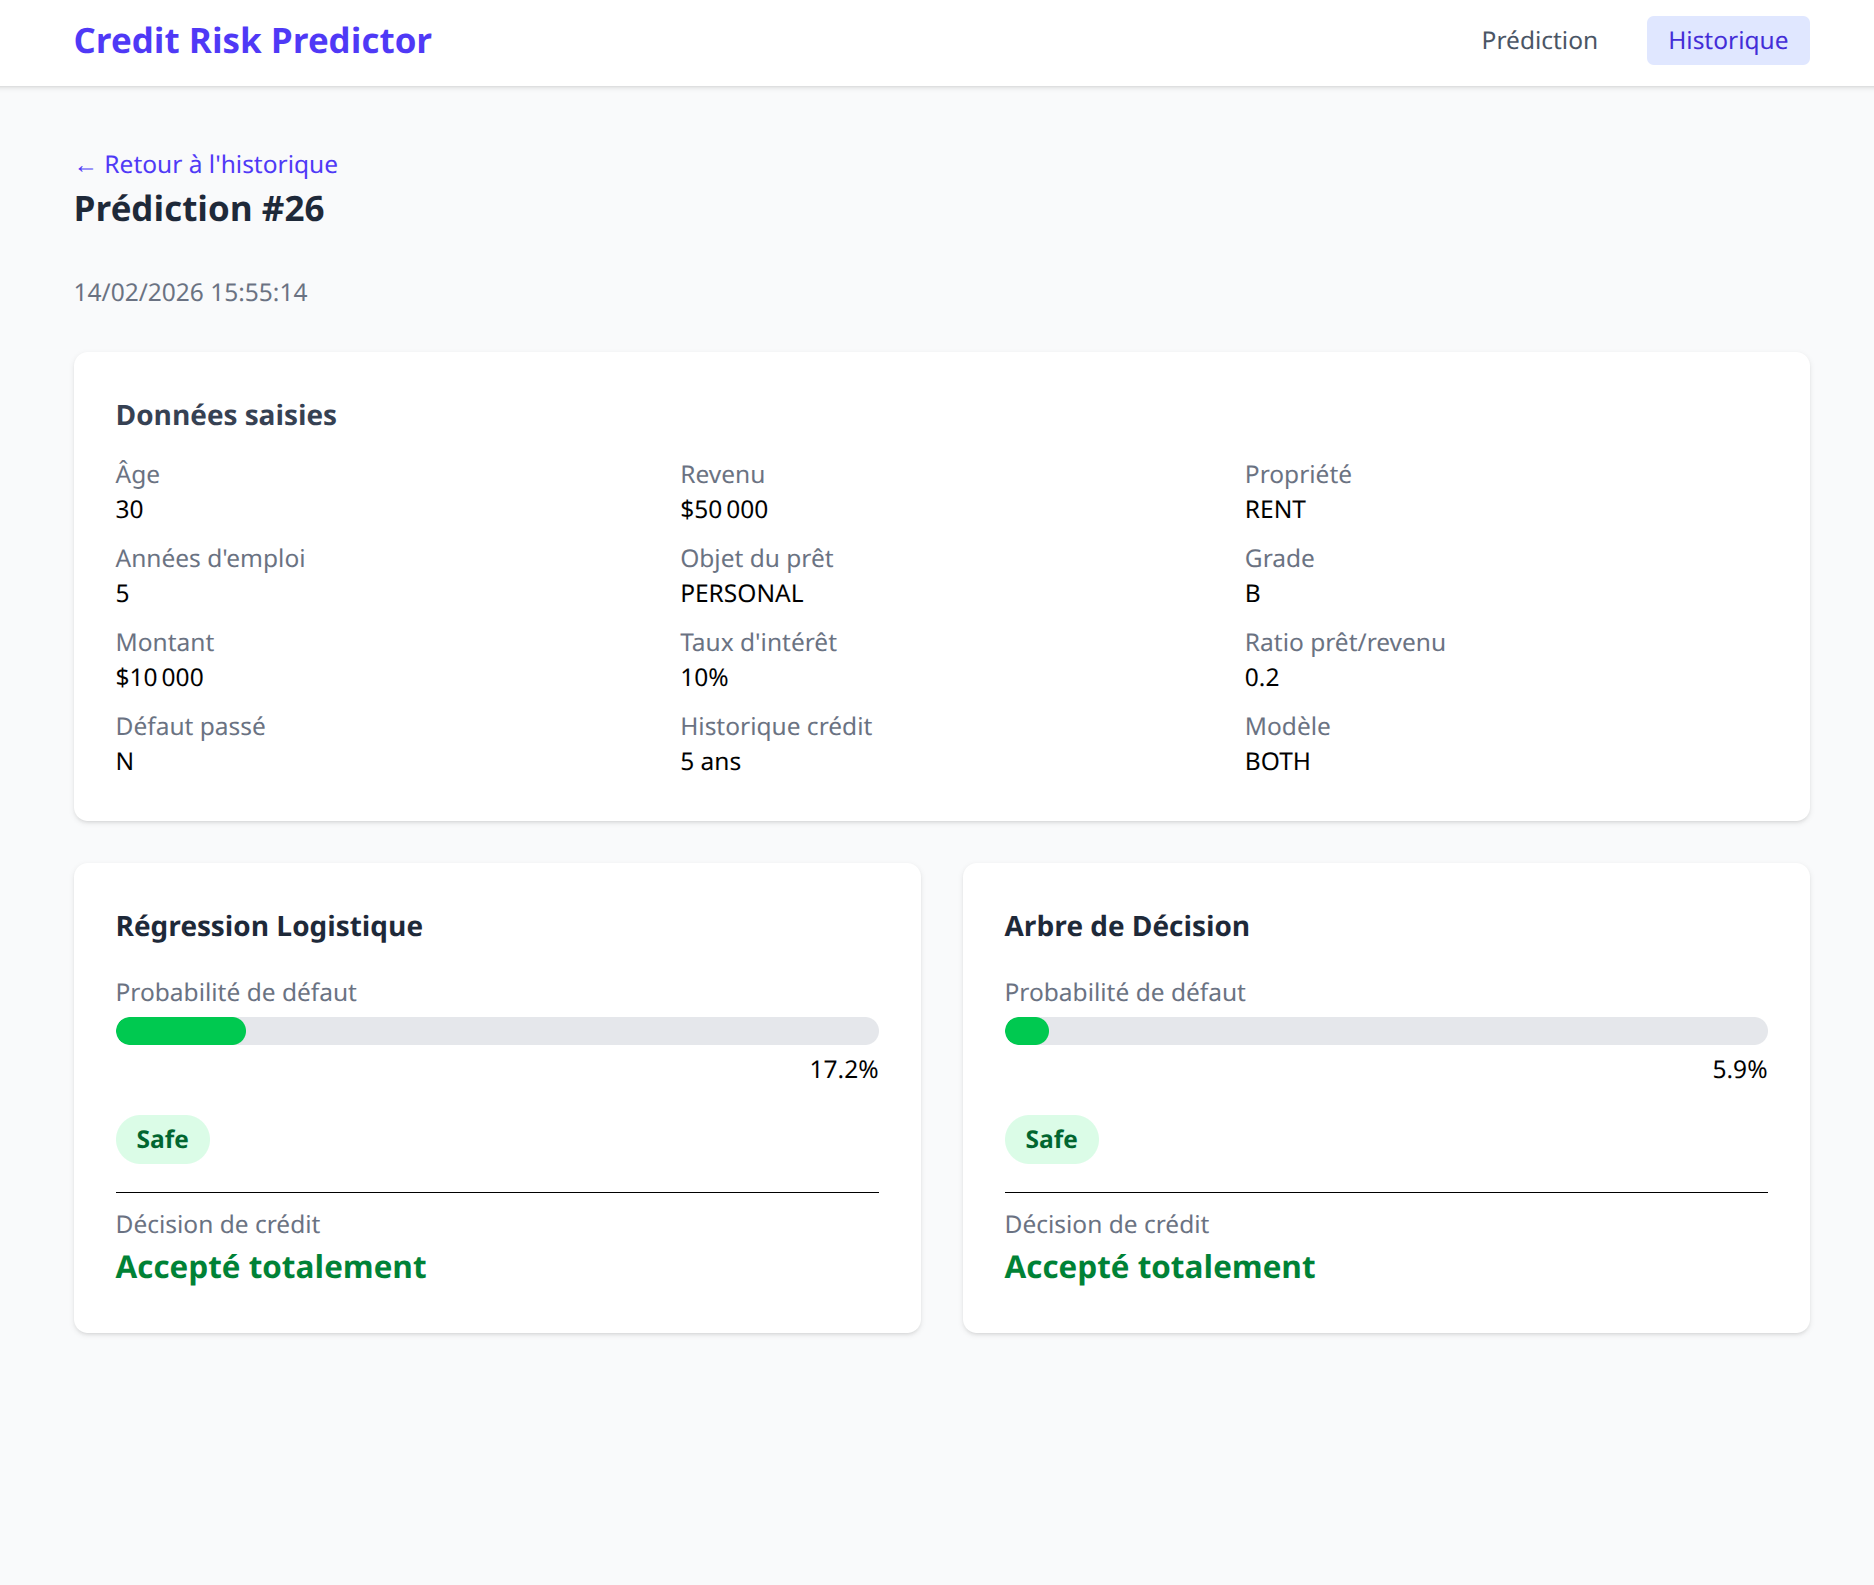
\includegraphics[width=\textwidth]{images/interface42}
    \caption{Détail d'une prédiction (DetailView) : données saisies et résultats des deux modèles.}
    \label{fig:interface-4}
\end{figure}

\begin{figure}[H]
    \centering
    \includegraphics[width=\textwidth]{"images/interface 5"}
    \caption{Vue complémentaire de l'interface web.}
    \label{fig:interface-5}
\end{figure}

% ────────────────────────────────────────────────────────────────────────────
\end{document}
